%%%%%%%%%%%%%%%%%%%%%%%%%%%%%%%%%%%%%%%%%%%%%%%
%
%    Shear localization in inelastic rate dependent shearing deformations
%
%                                                      by
%
%                    Th. Katsaounis,   Min-Gi Lee   and   A.E. Tzavaras
%
%                                          version May 2016, for Hyp2016 conference
%
%
%%%%%%%%%%%%%%%%%%%%%%%%%%%%%%%%%%%%%%%%%%%%%%%



\documentclass{beamer}

\usepackage{mathtools}
\usepackage{amsmath,amssymb,amsthm,psfrag,subfigure}
\usepackage{setspace}
\usepackage{color}
\usepackage{cancel}

%%%% macros from beamer.cls %%%%%%%%%%%%%%%%
  \usetheme{Boadilla}
  \usecolortheme{whale}
  \setbeamertemplate{footline}[frame number]
  \setbeamercovered{transparent}


%%%% my macros %%%%%%%%%%%%%%%%%%%%%%%%%%%%
  \def\red{\color{red}}
  \def\blue{\color{blue}}

  \def\bG{\bar{\Gamma}}
  \def\bS{\bar{\Sigma}}
  \def\bV{\bar{V}}
  \def\bU{\bar{U}}

\def\tr{\,\textrm{tr}\,}
\def\div{\,\textrm{div}\,}
\def\sgn{\,\textrm{sgn}\,}

\def\th{\tilde{h}}
\def\tx{\tilde{x}}
\def\tk{\tilde{\kappa}}


\def\bg{{\bar{\gamma}}}
\def\bv{{\bar{v}}}
\def\bth{{\bar{\theta}}}
\def\bs{{\bar{\sigma}}}
\def\bu{{\bar{u}}}
\def\bph{{\bar{\varphi}}}


\def\tg{{\tilde{\gamma}}}
\def\tv{{\tilde{v}}}
\def\tth{{\tilde{\theta}}}
\def\ts{{\tilde{\sigma}}}
\def\tu{{\tilde{u}}}
\def\tph{{\tilde{\varphi}}}

\def\dtg{{\dot{\tilde{\gamma}}}}
\def\dtv{{\dot{\tilde{v}}}}
\def\dtth{{\dot{\tilde{\theta}}}}
\def\dts{{\dot{\tilde{\sigma}}}}
\def\dtu{{\dot{\tilde{u}}}}
\def\dtph{{\dot{\tilde{\varphi}}}}

\def\dpp{\dot{p}}
\def\dqq{\dot{q}}
\def\drr{\dot{r}}
\def\dss{\dot{s}}

\def\ta{{\tilde{a}}}
\def\tb{{\tilde{b}}}
\def\tc{{\tilde{c}}}
\def\td{{\tilde{d}}}

\def\BO{{\mathcal{O}}}
\def\lio{{\mathcal{o}}}



\def\bx{\bar{x}}
\def\bm{\bar{\mathbf{m}}}
\def\K{\mathcal{K}}
\def\E{\mathcal{E}}
\def\del{\partial}
\def\eps{\varepsilon}

\newtheorem{proposition}{Proposition}


\begin{document}
\title[Localization ]{Localization in dynamic plasticity: \\ A study of parabolic regularizations  \\
of elliptic initial value problems}
% \title{{\LARGE Two-parameters family of focusing self-similar solutions in 1-d thermo-visco-plasticity}\\ {\small(Introduction to Geometric Singular Perturbation Theory)}}
\author{\vskip 5pt \small {Min-Gi Lee}\\ \vskip 5pt \scriptsize Applied Maths. \& Computational Science, KAUST, SA\\}
%\author{\vskip 5pt\Large {\underline{Thesis Defense}}}

\vskip 15pt
\institute{\scriptsize
Joint works with  \\ \textbf{\color{red}J. Olivier}, Universite de Marseilles, FR\\
\textbf{\color{cyan} Th. Katsaounis}, KAUST, SA \\
\textbf{\color{blue} A. Tzavaras}, KAUST, SA}

% \institute{\vskip 5pt joint with Athanasios Tzavaras \quad and \quad Thodoros Katsaounis\\}
\date{~}
\begin{frame}
  \titlepage
  \vskip -60pt
  \center
  {\small
  %{\scriptsize Summer School in Nonlinear Partial Differential Equations}\\
  {\scriptsize September 28th, 2017, Group Meeting}\\}
  %{\scriptsize Universit\"at Wien, Austria}\\
  %{\scriptsize Universit\"at Stuttgart, Stuttgart, Germany}\\
  %{\scriptsize  Texas A\&M University, U.S.}\\
%   {\scriptsize June 20th, 2017}\\}
%   {\scriptsize Group Meeting, KAUST}\\
%   {\scriptsize  Thuwal, Saudi Arabia}\\
%   {\scriptsize Octobor 13th, 2015}\\}
\end{frame}

\section{Introduction}

\begin{frame}\setstretch{1.4}\frametitle{Material instability}

Material instability in  solid mechanics :  A state loses its stability, typically a non-uniform deformation emerges

\bigskip

Examples
\begin{itemize}
\item nucleation in phase transitions
\item localization and shear bands, in various contexts
\begin{itemize}
\item[] compression of concrete blocks, granular materials
\item[] high strain-rate deformations of metals
\end{itemize}
\end{itemize}

\end{frame}

\begin{frame}
 \frametitle{Material Instability}
 \setstretch{1.5}
 \begin{itemize}
  \item Necking (Tensile Load)
   \begin{figure}
    \centering
      \includegraphics[height=2.5cm]{necking.eps} 
%      \caption{Typical stress-strain curve for metals}
    \end{figure} 
  \item Shear Band (Shear Load)
     \begin{figure}
    \centering
      \includegraphics[height=2.5cm,width=5cm]{sb2.eps} 
%      \caption{Typical stress-strain curve for metals}
    \end{figure} 
 \end{itemize}
 \vfill
\end{frame}



\begin{frame}
\frametitle{A Shear Band}
\setstretch{1.2}

  \begin{figure}
    \centering\includegraphics[height=3cm,width=4cm]{sb.eps}
  \end{figure}
%   \vspace{-5cm}
%  \begin{center}
%   \hspace{10pt} Shear Band in a Aluminum alloy
 % \end{center}

% \bigskip


A \underline{narrow layer of intense shearing} that develops when materials (metals, polymers, powders) are deforming at high strain rates.

{\scriptsize
\begin{itemize}
\item Typical shear band widths : $10-100 \mu m$
%\item High local values of shear strain : $5-100$
\item Ultra high local shear strain rates : $10^4/s - 10^6/s$
\item Local temperature rises several hundred degrees
%\item High propagation speeds : $\sim 1000m/s$
\item Not a crack : material preserves its integrability
%\item Shear Bands are  precursors to rupture
\end{itemize}
}

\vspace{0.2cm}
{\footnotesize
Experiments performed in experimental device Kolsky bar \\
\hfill {\footnotesize \color{red} groups of Duffy, Clifton - Brown 80's }
}
\end{frame}



\begin{frame}
 \frametitle{A Shear Band}
 \setstretch{1.5}
 \begin{minipage}{0.3\linewidth}
 \begin{figure}
    \centering
    {
      %\vspace{-5em}
      \includegraphics[height=2cm]{sb.eps} 
    } 
    \caption{Shear Band}
 \end{figure}
 \end{minipage}
  \hfill
 \begin{minipage}{0.6\linewidth}
 \begin{figure}
%     \subfigure[{\scriptsize UniformShear}]{
      \includegraphics[width=1.5cm,height=4cm]{uniformshear2.eps}
     \quad \quad \quad
%     \subfigure[Shear Localization]{
      \includegraphics[width=1.5cm,height=4cm]{shearband2.eps}
%     }
    \caption{Schematic sketch: uniform shear VS shear localization}
 \end{figure}
 \end{minipage}
 
 %Zener and Hollomon(1944) observed the formation of shear bands in the high speed deformation of metals, which are narrow zones shear localizes intensely.
 %\vfill
\end{frame}

\begin{frame}
\frametitle{Modeling adiabatic shear bands}

{\small 
1-d  {\blue shear motion} with {\red thermal effects}
\\
$y(x,t)$ displacement in shearing direction, $v = y_t$, $\gamma = y_x$
\\
 \begin{figure}
    \centering\includegraphics[height=1.5cm,width=10cm]{sbflow.eps}
    \caption{{Uniform shearing }  \hspace{0.2cm}  {\blue vs.}  \hspace{0.2cm} {\red shear band}}
  \end{figure}
  
\vspace{-0.2cm}
\begin{equation*}
  \begin{aligned}
    & v_{t} = \frac{1}{r}\ \sigma_{x}
    \\
    & \theta_{t} = \kappa \theta_{ x x}  +  \sigma \gamma_{t}
     \\
    & \gamma_{t} = v_{x}
  \end{aligned}
  \qquad \qquad
  \sigma = \varphi(\theta,\gamma)\gamma_t^n=\theta^{-\alpha} \gamma^m {\gamma_t}^n
\end{equation*}
non-dimensional numbers 
$\begin{cases}
 r &  \text{ratio of inertial versus viscous stresses}
\\
\kappa & \text{thermal diffusivity -- \color{red}{  $\kappa = 0$ adiabatic }}
\end{cases}$
\\
$\sigma$ is given by a {\color{cyan} power law } and expresses a flow rule on a yield surface

 }

\end{frame}

\begin{frame}
 \setstretch{1.5}
 \frametitle{Uniform Shearing Solutions}
 Regardless of the precise form of $\varphi(\theta,\gamma)$, the model admits {\red uniform shearing solutions},
 \begin{align*}
  v_s(x) = x, \quad \gamma_s(t) = t + \gamma_0, \quad \sigma_s = \sigma_s(t), \quad \theta_s=\theta_s(t),\quad \text{$\gamma_0$ a constant}.
 \end{align*}
 
  \begin{figure}
    \center
    \psfrag{stress}{\hskip -3em stress $\sigma$}
    \psfrag{strain}{strain $\gamma$}
    \psfrag{phi}{$\sigma^{'}( \gamma ) < 0$}% = \frac{1}{\gamma}$}
    \includegraphics[height=2.8cm]{uniformshear.eps}
    \caption{{\footnotesize Uniform shearing.}}
  \end{figure}
  
 %At the core of understanding of the model is the question whether this uniform motions go astray developing the material instability.   
\end{frame}

%%%%%%%%%%%%%%%%%%
\begin{frame}
\frametitle{Uniform shearing solutions}

%\vskip-1cm
{\small 
  \begin{align*}
     v_s  &= x \\
    \gamma_s (t)  &= t + \gamma_0 \\
     \dot \theta_s (t)  &= \sigma_s (t) =  {\theta_s (t) }^{-\alpha}(t+\gamma_0)^m
     \\
%     \left\{\theta_0^{\alpha+1}+\frac{\alpha+1}{m+1}\left[(\gamma_0+t)^{m+1}
%     -\gamma_0^{m+1}\right]\right\}^{\frac{1}{\alpha+1}} \\
%    \sigma_s (t)  &= {\theta_s (t) }^{-\alpha}(t+\gamma_0)^m
  \end{align*}



\vskip-1.2cm 

\begin{figure}
    \centering\includegraphics[height=4cm,width=5cm]{HardSoft.eps}
    \caption{ $\sigma_s (t)$ \; vs \; $t$}
  \end{figure}
  \vskip-15pt
  $ \sigma_s (t)$ initially increases (hardening) but eventually decreases (softening) 

}

\end{frame}

\begin{frame}
 \frametitle{Theme: parabolic regularization of ill-posed problem.}
 \setstretch{1.2}
 {\blue \sc Summary of models}:  
 
 {\color{cyan} power law }
 \vskip -0.1em
 {\scriptsize
\begin{equation*}
  \begin{aligned}
    & v_{t} =  \sigma_{x}
    \\
    & \theta_{t} = \kappa \theta_{ x x}  +  \sigma \gamma_{t}
     \\
    & \gamma_{t} = v_{x}
  \end{aligned}
  \qquad \qquad
  \sigma = \theta^{-\alpha} \gamma^m {\gamma_t}^n
\end{equation*}
}
 {\color{cyan} exponential law }
 \vskip -0.1em
 {\scriptsize
\begin{equation*}
  \begin{aligned}
    & v_{t} =  \sigma_x 
    \\
    & \theta_{t} = \kappa \theta_{ x x}  +  \sigma v_x
  \end{aligned}
  \qquad \qquad
  \sigma =e^{-\alpha \theta }  {v_x}^n \, , \quad {\textstyle \alpha > 0, \; n> 0}
\end{equation*}
 }
{\small Underlying issues:

\begin{itemize}
\item  dependence of viscosity on the temperature

\item parabolic regularization of an elliptic IVP
\end{itemize}

We focus on the constitutive law of the form
  \vskip -10pt
  
$$\sigma=\varphi(\theta,\gamma){\red (\gamma_t)^n}, \quad 0<n\ll1$$
% where $\varphi(\theta,\gamma)$ is such that {\blue net softening response} is exhibited. This effect competes with the regularization due to the {\blue small rate-dependency}.
%  \vfill
% The ill-posed problem is regularized by small viscosity to result in the yet orderly instability that is without growth of high frequency oscillations.
%  \vfill
}
\end{frame}

\begin{frame}
 \frametitle{$n=0$: Hadamard Instability}%Stress-strain curve}
 \setstretch{1.5}
 \begin{figure}
    \centering
    \center
    \psfrag{s}{\scriptsize stress $\sigma(\gamma)$}
    \psfrag{g}{\scriptsize strain $\gamma$}
%     \psfrag{phi}{\scriptsize  $\varphi^{'}( \gamma ) < 0$}% = \frac{1}{\gamma}$}
    \includegraphics[width=5.5cm]{phi2.eps} 
    \caption{Typical stress-strain curve for metals in uniaxial tensile test.}
 \end{figure} 
 Blue dotted box corresponds to the elastic regime; red dotted box is the regime of instability.
 \vfill
\end{frame}


\begin{frame}
 \frametitle{Softening and the Loss of Hyperbolicity}
 \setstretch{1.5}
 1D Elastodynamics system.
 \begin{align*}
  \begin{pmatrix}
   v_t\\ \gamma_t
  \end{pmatrix}
  = \begin{pmatrix}
   0 &\sigma'(\gamma)\\ 1 & 0
  \end{pmatrix} 
  \begin{pmatrix}
   v_x\\ \gamma_x
  \end{pmatrix}.
 \end{align*}
 \vfill
 \begin{itemize}
  \item $\sigma'(\gamma)<0$ results in the loss of hyperbolicity.
  \item Model predicts the exponential growth of oscillations in the initial-value-problem: {\blue Hadamard Instability}.
 \end{itemize}
\end{frame}

\begin{frame}
 \frametitle{Adiabaticity and Thermal Softening}
 \setstretch{1.5}
  In Adiabatic process, heat accumulates.  
  
  Suppose the inviscid problem with phenomenological law
 $$\sigma=\varphi(\theta,\gamma)=\theta^{-\alpha}\gamma^m, \quad \alpha>0.$$
 Then, the Energy equation reads
 \begin{align*}
  \theta_t = \theta^{-\alpha}\gamma^m\gamma_t \quad \Longleftrightarrow \quad 
  \left(\frac{\theta^{1+\alpha}}{1+\alpha}\right)_t = \left(\frac{\gamma^{1+m}}{1+m}\right)_t
 \end{align*}
 Modulo Initial data, only one of the temperature and strain plays the role.
 
 Roughly, $\theta\sim \gamma^{\frac{1+m}{1+\alpha}}$ or
 $$\sigma \sim \gamma^{\frac{\red-\alpha+m}{1+\alpha}}.$$
 \vfill
\end{frame}

\begin{frame}
 \frametitle{Net Softening and the Loss of Hyperbolicity}
 \setstretch{1.5}
\begin{equation} \label{eq:transport}
 \begin{pmatrix} \gamma_t \\ \theta_t \\ v_t \end{pmatrix} = \underbrace{
 \begin{pmatrix}
  0 & 0 & 1\\
  0 & 0 & \theta^{-\alpha}\gamma^m \\
  m\theta^{-\alpha}\gamma^{m-1} & -\alpha\theta^{-\alpha-1}\gamma^m & 0\end{pmatrix}}_\text{$\triangleq B$}
  \begin{pmatrix} \gamma_x \\ \theta_x \\ v_x \end{pmatrix}. 
\end{equation}
% {\scriptsize
% \begin{align*}
%  \det\big(B-\mu\textrm{I}\big) &= -\mu\big(\mu^2+\theta^{-\alpha}\gamma^{m-1}\Big(\frac{\alpha-m}{1+\alpha}+\alpha \frac{\gamma_0(x)^{1+m} - \frac{1+m}{1+\alpha}\theta_0(x)^{1+\alpha}}{\theta^{1+\alpha}}\Big),
% \end{align*}
% }
\vfill
$-\alpha+m<0$ implies the loss of hyperbolicity.
%   \item $\sigma'(\gamma)<0$ results in the loss of hyperbolicity.
%   \item Model predicts the exponential growth of oscillations in the initial-value-problem: {\blue Hadamard Instability}.
%  \end{itemize}
\end{frame}

\begin{frame}
 \frametitle{Loss of Hyperbolicity and High oscillations}
 \setstretch{1.5}
 \begin{itemize}
  \item High oscillations are amplified exponentially in Hadamard instability,
%   \item Mismatch in model and material instability.
  \item while such a high oscillations are not observed in the experiments. %Rather, the coherent localization is observed.
  \item The parabolic regularization can accounts for that.
 \end{itemize}
 \vfill
\end{frame}



\begin{frame}
 \frametitle{Cf. Stability results in large viscous regime}
 \setstretch{1.4}
{\color{cyan} power law }
\begin{equation*}
  \begin{aligned}
    & v_{t} =  \sigma_{x}
    \\
    & \theta_{t} =   \sigma \gamma_{t}
     \\
    & \gamma_{t} = v_{x}
  \end{aligned}
  \qquad \qquad
  \sigma = \theta^{-\alpha} \gamma^m {\gamma_t}^n
\end{equation*}
 \begin{itemize}
  \item $m=0$, $-\alpha+n>0$ :  USS is globally asymptotically stable {\footnotesize (Daefermos and Hsiao 1983, Tzavaras 1992)}.
  \item {\blue We expect similar for $-\alpha+m+n>0$ but we have not proved yet.}
 \end{itemize}

  
  \vfill
\end{frame}

\begin{frame}\frametitle{An asymptotic mechanism for localization}
\setstretch{1.4}
{\color{cyan} power law }
\begin{equation*}
  \begin{aligned}
    & v_{t} =  \sigma_{x}
    \\
    & \theta_{t} =   \sigma \gamma_{t}
     \\
    & \gamma_{t} = v_{x}
  \end{aligned}
  \qquad \qquad
  \sigma = \theta^{-\alpha} \gamma^m {\gamma_t}^n
\end{equation*}

% \vspace{1.5 cm}

{\color{blue} uniform shear solution }

\begin{equation*}
  \begin{aligned}
  v_s = x \quad \theta_s = \theta_s (t) \quad \gamma_s = t + \gamma_0 \quad \sigma_s = \sigma_s (t)
  \end{aligned}
   \end{equation*}
   
% \vspace{0.5 cm}

{\color{red} a recurring theme in this problem} \\
stability analysis of a time-dependent solution leads to non-autonomous systems



\end{frame}

%%%%%%%%%%%%%%%%%%
\begin{frame}\setstretch{1.2}\frametitle{}

{\small
Consider the power law, with adiabatic conditions ($\kappa = 0$) and  introduce
the {\color{red} relative perturbation variables} and the {\color{blue} change of time scale}
$$
\dot \tau = \sigma_s (t)  \Longleftrightarrow t = \hat t (\tau)
$$
\begin{alignat*}{2}
v_x = u(x,t) &= U \big ( \frac{x}{\sqrt{R}} , \frac{\tau(t)}{R} \big ) \qquad \qquad
\theta (x,t) &&= \theta_s(t) \Theta \big ( \frac{x}{\sqrt{R}} , \frac{\tau(t)}{R} \big )
\\
\gamma (x,t) &= \gamma_s(t) \Gamma \big ( \frac{x}{\sqrt{R}} , \frac{\tau(t)}{R} \big )
\qquad
\sigma (x,t) &&= \sigma_s(t) \Sigma \big ( \frac{x}{\sqrt{R}} , \frac{\tau(t)}{R} \big )
\end{alignat*}
to obtain the {\color{blue} relaxation system}. The uniform shear solution is mapped
to the equilibrium point  $(1,1,1,1)$

\smallskip
$$
\begin{aligned}
U_\tau &= \Sigma_{xx}
\\
{\textstyle \frac{\bar \theta_s}{R}} \; \Theta_\tau &= \Sigma U - \Theta
\\
{\textstyle \frac{\bar \sigma_s \bar   \gamma_s}{R}} \; \Gamma_\tau &= U - \Gamma
\\
\Sigma &= \Theta^{-\alpha} \Gamma^m U^n
\end{aligned}
$$

}

\end{frame}


%%%%%%%%%%%%%%%%%%
\begin{frame}\setstretch{1.4}\frametitle{}

{\small

An asymptotic procedure analogous to the {\color{blue} Chapman-Enskog expansion } gives
for $R >> 1$
\begin{alignat*}{2}
&{\color{blue} O\Big ( \frac{1}{R} \Big )  } \qquad 
 &&\partial_\tau U = \partial_{xx} \Big (    U^p \Big )
  \\
 &  &&
\\
&{\color{blue} O\Big ( \frac{1}{R^2} \Big ) } \qquad 
 &&\partial_\tau U = \partial_{xx} \Big (   U^p  +  \frac{\lambda }{R} ( \tau+1) 
                                                                                         \, U^{p-1} \partial_{xx} U^p  \Big )
\end{alignat*}
where $\lambda$ positive constant and 
\vspace{0.5cm}

\centerline{ {\color{blue} $p = \frac{-\alpha + m +n}{1+\alpha}$  } }
\begin{itemize}
\item[] {\color{blue} $p > 0$  } \quad 2$^{nd}$ order equation is stable
\item[] {\color{blue} $p < 0$  } \quad 2$^{nd}$ order eq. unstable (linearly ill-posed), \\
       \qquad \qquad                  4$^{th}$ order eq. stable regularization ($\lambda>0$) \\
      \qquad \qquad \qquad           of  a backward parabolic equation
\end{itemize}

\vskip -10pt
\hfill {\footnotesize \color{red} Katsaounis-T. 09 }
}

\end{frame}

% %
% %
% %
% \begin{frame}\setstretch{1.4}\frametitle{ Towards a mathematical theory for shear bands - the exp model}
% 
% 
% \begin{itemize}
% \item{}  To outline the "complete" picture for a paradigm :  the {\blue exp}  model
% 
% \begin{itemize}
% 
% \item{} Linearized stability
% \item{} Nonlinear model - A scenario for localization
% \item{} A class of  solutions exhibiting localization 
% \item[]  Hadamard instability vs Localization
% 
% \end{itemize}
% 
% 
% \end{itemize}
% 
% 
% Paradigm:  {\color{blue} exponential law }
% \begin{equation*}
%   \begin{aligned}
%     & v_{t} =  \sigma_x 
%     \\
%     & \theta_{t} = \kappa \theta_{ x x}  +  \sigma v_x
%   \end{aligned}
%   \qquad \qquad
%   \sigma =e^{-\alpha \theta }  {v_x}^n \, , \quad {\textstyle \alpha > 0, \; n> 0}
% \end{equation*}
% 
% 
% \end{frame}
% 
%%%%%%%%%%%%%%%%%%



%%
%%%%   Numerical simulations -  Slides 
%
%
%%%%%%%%%%%%%%%%%%


%
%
%
% Suggestions of numerical runs
%
%
%%%%%%%%%%%%%%%%%%
% \section{linearized theory}
% \begin{frame}\setstretch{1.4}\frametitle{\small what is special in the exp model ?}
% 
% 
% \begin{equation*}
% \begin{aligned}
%   & v_{t} = \sigma_{x},\\
%   & \sigma = e^{-\alpha \theta } v_x^{n}   \\
%   & \theta_{t} = \kappa \theta_{x x} + \sigma v_x 
%   \end{aligned}
% \qquad \qquad  \mbox{ {\blue uniform solution} }
% \left \{
% \begin{aligned}
%   & v_s  = x \\
%   & \theta_s = \frac{1}{\alpha} \ln \left ( \alpha t + c_0 \right )  
%   \\
%   & \sigma_s = e^{- \alpha \theta_s} = \frac{1}{\alpha t + c_0 }
%  \end{aligned}
%  \right .
% \end{equation*}
% 
% \vspace{1cm}
% 
% \begin{itemize}
% \item in general non-autonomous issues appear
% 
% \item here, the adiabatic case $\kappa = 0$ leads to an autonomous problem
% 
% \end{itemize}
% 
% \end{frame}
% 
% %%%%%%%%%%%%%%%%%%
% \begin{frame}\setstretch{1.4}\frametitle{\small relative perturbation and rescaling}
% 
% 
% {\small 
% \begin{equation*}
% \begin{aligned}
%   & V =  V(x,\tau(t) ) \\
%   & \theta = \theta_s (t) + \Theta (x,\tau(t) )   \\
%   & \sigma = \sigma_s (t)  \, \Sigma (x,\tau(t) ) 
%   \end{aligned}
%   \qquad
%   \text{with} 
%   \quad 
%   \dot \tau (t) = \sigma_s (t) = \frac{1}{\alpha t + c_0}
% \end{equation*}
% for {\color{red} $U = V_x$ } we  obtain the system 
% 
% \begin{equation*}
% \begin{aligned}
%   & U_{\tau} =  \, \Sigma_{x x},\\
%   & \Theta_{\tau} =  {\red \kappa  \, e^{\alpha \tau}  \, \Theta_{x x}  }+  ( \Sigma U - 1) \\
%   & \Sigma = e^{-\alpha \Theta } U^{n}   
%     \end{aligned}
% \end{equation*}
% 
% 
% \vskip0.5cm
% uniform shear is mapped to equilibrium :  $U_0 =1, \Theta_0 = 0, \Sigma_0=1$ \\
% \smallskip
% {\red For $\kappa = 0$ - adiabatic - the system is autonomous }
% }
% 
% \end{frame}
% 
% %%%%%%%%%%%%%%%%%%
\begin{frame}\setstretch{1.2}\frametitle{Linearized analysis of exp model}
{\small


\begin{equation*}
\begin{aligned}
  & U =  1 + \delta u + O(\delta^2) ,\\
  & \Sigma = 1 + \delta s + O(\delta^2),     \\
  & \Theta =  1 + \delta \theta  + O(\delta^2)
    \end{aligned}
\end{equation*}

\vspace{1cm} 

{\color{blue}Linearized stability analysis} for perturbation $(u, \theta, s)$


\begin{equation*}
\begin{aligned}
  \frac{\del u }{\del \tau}  &=  \Big ( n \ u_{ x x}  - \alpha \theta_{x x} \Big ) ,\\
  \frac{\del \theta }{\del \tau} &=\kappa e^{\alpha \tau} \theta_{xx}  +
   \Big ( -\alpha \theta + (n+1) u \Big )   \\
    s  & = -\alpha \theta + n u     \\
 \end{aligned}
\end{equation*}
with boundary conditions
$$
u_{x} (0,\tau) = u_{x} (\pi, \tau) = 0 \quad 
\theta_{x} (0,\tau) = \theta_{x} (\pi,\tau) = 0 
$$
%admits solutions in form of  {\color{cyan} Fourier modes}
%\begin{equation*}
%\begin{aligned}
%  u (x,\tau) = \hat v_j (\tau) \cos ( j x)  ,\\
%  \theta (x,\tau) = \hat \xi_j (\tau)   \cos ( j x)   \\
% \end{aligned}
%\end{equation*}
%which satisfy {\color{cyan} a non-autonomous system} when $\kappa \ne 0$.

}
\end{frame}


%%%%%%%%%%%%%%%%%%
\begin{frame}\setstretch{1.4}\frametitle{Linearized analysis of exp model $\kappa = 0$}


{\small 

\begin{itemize}
\item
$\kappa = 0$, $n = 0$  -  {\color{red} Hadamard Instability} \\
$$
\lambda_{j +}  > 0 >  \lambda_{j -}  \quad \forall j
$$
with unstable modes
$$
\theta_j (x,t) \sim \cos (j  x) e^{\lambda_{j +} \tau (t)} \, , \qquad \lambda_{j +} \sim j 
$$


\item
$\kappa = 0$, $n > 0$  -  {\color{red} Turing Instability} \\
$$
\lambda_{j +}  > 0 >  \lambda_{j -}  \quad \forall j
$$
with unstable modes
$$
\theta_j (x,t) \sim \cos (j  x) e^{\lambda_{j +} \tau (t)} \, , \qquad \lambda_{j +} \nearrow \tfrac{\alpha}{n}
$$


%The behaviour  is an example of {\color{blue} Turing instability}:
%$$
%\dot x = (A + B) x \quad \mbox{ with $Re(A) < 0$, $Re (B) < 0$ but  $Re(A+B) > 0$}.
%$$

\end{itemize}
}

\end{frame}

\begin{frame}\setstretch{1.2}\frametitle{Linearized analysis of power law model $\kappa = 0$}
{\small

\begin{align*}
 U &= 1 + \delta U_1 + \mathcal{O}(\delta^2), & \Gamma &= 1 + \delta \Gamma_1 + \mathcal{O}(\delta^2), \\
 \Sigma &= 1 + \delta \Sigma_1 + \mathcal{O}(\delta^2), & \Theta &= 1 + \delta \Theta_1 + \mathcal{O}(\delta^2).
\end{align*}
{\color{blue}Linearized stability analysis} for perturbation $(u, \theta, s)$
\begin{equation} \label{eq:linsystem}
 \begin{aligned}
  \partial_\tau U_1 &= \Sigma_{1xx},\\
  \partial_\tau\Gamma_1 &= \frac{1}{\tau}\frac{1+\alpha}{1+m}(U_1-\Gamma_1),\\
  \partial_\tau\Theta_1 &= \frac{1}{\tau}\Big(\Sigma_1+ U_1 -\Theta_1\Big),\\
  0&=\Sigma_1 + \alpha\Theta_1 -m\Gamma_1 - nU_1 .
 \end{aligned}
\end{equation}


with boundary and constraint conditions
\begin{equation} \label{eq:linbdry}
 \Sigma_{1x}(\tau,0)=\Sigma_{1x}(\tau,1)=0, \quad \int_0^1 U_1(t,x) \: dx = 0.
\end{equation}
%admits solutions in form of  {\color{cyan} Fourier modes}
%\begin{equation*}
%\begin{aligned}
%  u (x,\tau) = \hat v_j (\tau) \cos ( j x)  ,\\
%  \theta (x,\tau) = \hat \xi_j (\tau)   \cos ( j x)   \\
% \end{aligned}
%\end{equation*}
%which satisfy {\color{cyan} a non-autonomous system} when $\kappa \ne 0$.

}

\end{frame}


% 
% %%%%%%%%%%%%%%%%%%%
% %\begin{frame}\setstretch{1.4}\frametitle{\small linearized analysis $\kappa > 0$ w. frozen in time coefficients}
% %
% %
% %
% %\begin{itemize}
% %
% %
% %\item
% %$\kappa > 0$  -  {\color{red} Effect of diffusion is to stabilize the system} 
% %\begin{itemize}
% %\item
% % eigenvalue analysis of system with frozen in time coefficients
% %\begin{itemize}
% %\item The eigenvalues are always real
% %\item There is one positive eigenvalue for the $j^{th}$-mode iff
% %$$
% %j^2 n \kappa  - \alpha < 0 
% %$$
% %where  $j = 1, 2, ...$ is the Fourier mode.
% %\end{itemize}
% %
% %\item The behaviour (for $\kappa$ small) is again an example of
% %{\color{blue} Turing instability}
% %
% %\item For $\kappa n > \alpha$ all modes are stable
% %
% %\end{itemize}
% %\end{itemize}
% %
% %\end{frame}
% %
% 
% 
% %%%%%%%%%%%%%%%%%%%
% \begin{frame}\setstretch{1.4}\frametitle{\small linearized analysis of non-autonomous system $\kappa \ne 0$}
% 
% 
% {\small
% 
% \begin{equation*}
% \begin{aligned}
%   \frac{\del u }{\del t}  &=  \sigma_s(t)  \Big ( n \ u_{ x x}  - \alpha \theta_{x x} \Big ) ,\\
%   \frac{\del \theta }{\del t} &=\kappa  \theta_{xx}  +
%    \sigma_s (t) \Big ( -\alpha \theta + (n+1) u \Big )   \\
%  \end{aligned}
% \end{equation*}
% 
% \bigskip
% 
% %One shows by energy estimates
% %$$
% %\frac{d}{dt} \int \frac{A}{2} u^2 + \frac{1}{2} \theta^2 dx \le  ( A \sigma_s(t) - \kappa ) \int \theta_x^2 dx \le 0
% %$$
% %provided $t > T$ such that $A \sigma_s(t) \le \kappa$.
% %Also that
% %$$
% %\int \Big ( \frac{1}{2} u^2 + \frac{B}{2} \theta^2 \Big ) (x,t) dx  
% %\le e^{C_B t} \int \Big ( \frac{1}{2} u^2 + \frac{B}{2} \theta^2 \Big ) (x,0) dx \quad t \ge 0
% %$$
% 
% \bigskip
% 
% \begin{itemize}
% \item analysis of solution of non-autonomous system in $L^2$
% \item 
% {\color{blue} Asymptotic stability }
% Perturbations  grow initially but after a point in time the effect of thermal diffusion
% takes over and perturbations decay to zero. 
% 
% 
% \end{itemize}
% }
% 
% 
% \end{frame}
% %
% %
% %
% %%%%%%%%%%%%%%%%%%%
% %\begin{frame}\setstretch{1.4}\frametitle{\small Simulations - metastability for the  nonlinear system}
% %
% %
% %\vspace{0.5 cm}
% %  \begin{figure}
% %    \centering 
% %    \includegraphics[height=6cm,width=12cm]{Vmtstb}    
% %\caption{velocity $v$  vs $t$  --- $\kappa = 0.5$, $\alpha = 0.5$, $n = 0.05$}
% %   \end{figure}
% %\end{slide}
% %%
% %%
% %%
% %%
% %{}
% %\vspace{0.5 cm}
% %  \begin{figure}
% %    \centering 
% %       \includegraphics[height=6cm,width=12cm]{Qmtstb}    
% %\caption{temperature $\theta$ vs $t$  --- $\kappa = 0.5$, $\alpha = 0.5$, $n = 0.05$}
% %   \end{figure}
% %
% %\end{frame}
% %
% %
% %
% %  The nonlinear Arrhenius model
% %
% %%%%%%%%%%%%%%%%%%
% 
% 
% 
% 
% 
% \begin{frame}
%  \frametitle{Rate sensitivity $0<n\ll1$}
%  \setstretch{1.5}
%  Consider a rate-dependent stress
%  $$\sigma=\varphi(\theta,\gamma){\red (\gamma_t)^n}.$$
%  
%  We consider a singularly perturbed problem from its inviscid problem in the above form.
%  \vfill
% \end{frame}




% \begin{frame}
%  \frametitle{Parametric study of instability regime}
%  \setstretch{1.3}
%  \begin{figure}
%     \centering
%     \center
%     \psfrag{s}{\scriptsize stress }
%     \psfrag{g}{\scriptsize strain }
% %     \psfrag{phi}{\scriptsize  $\varphi^{'}( \gamma ) < 0$}% = \frac{1}{\gamma}$}
%     \includegraphics[width=2.5cm]{phi3.eps} 
%     \vskip -15pt
%      \caption{Instability Regime}
%     \end{figure} 
%  \vskip -5pt
%  We study the instability {\blue (competition between Hadamard Instability and Viscosity)} during the plastic deformation that effectively takes places in the red-dotted box, with the following form of the constitutive law
%  \begin{align}
%   \sigma &= \sigma(\gamma,\theta)(\gamma_t)^n=\theta^{-\alpha}\gamma^m(\gamma_t)^n, 
%  \end{align}%\footnote[frame]{J.W. Hutchinson and K.W. Neale (1977), Tzavaras (1991,1992)}.
%  with {\red $-\alpha +m+n<0$}, where $\alpha>0$, $m>-1$, $n>0$.\footnote[frame]{J.W. Hutchinson and K.W. Neale (1977), Tzavaras (1991,1992)}
% \end{frame}
% 
% 
% \begin{frame}
%  \frametitle{Adiabatic shear bands}
%  \setstretch{1.5}
%  Important features to recap:%observed during the development of localizing singularity are :
%  \vfill
%  \begin{enumerate}
% %   \item  is triggered.
%   \item The role of strain rate $\gamma_t$ falls into two folds:
%   \begin{enumerate}
%    \item It enters in the constitutive law%: dynamics depends on the rate.
%    \item High speed rate makes the loading condition close to {\it Adiabatic}; not enough time for heat to diffuse out.
%   \end{enumerate}
%   \item Albeit extremely fast development of singularity, the process is orderly: growths of oscillations are not observed and the localization occurs in {\red coherent} fashion.
%  \end{enumerate}
%  \vfill
% \end{frame}
\begin{frame}\setstretch{1.4}\frametitle{\small Numerical simulations  for the exponential model - $\kappa = 0$}

\begin{figure}
\centering
\includegraphics[height=3cm,width=8cm]{Arr_Vx.eps}
\caption{$v_x(\gamma_{t})$ in log-scale: evolution (left), final time (right)}
\label{arvx}
\end{figure}
%
\vspace{-0.5cm}
%
\begin{figure}
\centering
\includegraphics[height=2.8cm,width=8cm]{Arr_Stress.eps}
\caption{$\sigma$ : evolution (left), final time (right)}
\label{arstress}
\end{figure}
\end{frame}

\begin{frame}
\setstretch{1.3}
% \frametitle{1D Thermo-Visco-Plasticity of Shear Deformation}
\frametitle{1D rate-dependent thermo-plastic shear deformation}
%   \vskip 5pt
    \begin{minipage}{0.31\linewidth}
    \begin{figure}
    \centering
    \psfrag{Y}{\scriptsize $Y(t,x)$}
    \psfrag{y}{\scriptsize $y$}
%     \psfrag(x){\scriptsize $x$}
    \includegraphics[width=3cm]{shear1.eps}
    \end{figure}
%     \caption{The Specimen is under deformation in $y$-direction in $xy$-plane. } \label{fig:1}
      {\scriptsize
    \begin{equation*} %\label{eq:vars}
    \begin{aligned}
    \gamma(t,x) &: \text{plastic strain}\\
    \gamma_t(t,x) &: \text{strain rate}\\
    v(t,x) &: \text{vertical velocity}\\
    \theta(t,x) &: \text{temperature}\\
    \sigma(t,x) &: \text{stress}
    \end{aligned}
    \end{equation*}
    in $(t,x)\in \mathbb{R}^+ \times \mathbb{R}$}
    \end{minipage}
    \begin{minipage}{0.61\linewidth}
      \begin{equation*} %\label{system0}
        \begin{aligned}
          \partial_t v &= \partial_x\Big(\sigma(\gamma,\gamma_t,\theta)\Big) & &\text{({\blue Momentum balance})}, \\
          \partial_t \theta &= \sigma\partial_x v + \cancel{\red k\theta_{xx}} & &\text{({\blue Adiabatic Energy balance})},\\
          \partial_t \gamma &= \partial_x v & &\text{({\blue Kinematic compatibility})},\\
          \sigma  &= \sigma(\gamma,\gamma_t,\theta) & &\text{({\blue Constitutive Law})}\\
        \end{aligned}
      \end{equation*}
       subject to %\\
%       $v=\partial_t Y(t,x)$ is a {\blue velocity} in $y$-direction, \\
%       $\gamma=\partial_x Y(t,x)$ is a {\blue shear strain}.% and $\sigma(\gamma,\gamma_t,\theta)$ is a constitutive law for the {\blue shear stress}. 
      \vskip 5pt
      
      Initial conditions
      
      {\scriptsize $\gamma(0,x) = \gamma_0(x)$, $v(0,x) = v_0(x)$, $\theta(0,x) = \theta_0(x)$,} 
      
      Boundary velocity conditions.
      
%       {\scriptsize $v(t,x) \rightarrow f^-(t)$ as $x \rightarrow -\infty$, $v(t,x) \rightarrow f^+(t)$ as $x \rightarrow \infty$.}
      {\scriptsize $v(t,x) \rightarrow f^\pm(t)$ as $x \rightarrow \pm\infty$.}
    \end{minipage}
\end{frame}

\begin{frame}
 \frametitle{Perturbative features in viscous problem}
 Viscous problem with {\scriptsize {\red $-\alpha +m+n<0$}, $0<n\ll1$.}
 \setstretch{1.5}
 \begin{align*}
  v_t &= \big(\theta^{-\alpha}\gamma^m {\red (v_x)^n}\big)_x,\\
  \left(\frac{\theta^{1+\alpha}}{1+\alpha}\right)_t &= \left(\frac{\gamma^{1+m}}{1+m}\right)_t{\red (\gamma_t)^n},\\
  \gamma_t&=v_x,
 \end{align*}
 %Inviscid Adiabatic Shear flow is essentially of $2$-variables. 
 We view above system as the singularly perturbed one from the inviscid system.
  \vfill
 \begin{enumerate}
  \item Singularly perturbed:
  $v_t = \big(\theta^{-\alpha}\gamma^m {\red (v_x)^n}\big)_x.$
  \item Regularly perturbed:
  $ \left(\frac{\theta^{1+\alpha}}{1+\alpha}\right)_t = \left(\frac{\gamma^{1+m}}{1+m}\right)_t{\red (\gamma_t)^n}.$
 \end{enumerate}
\end{frame}

\begin{frame}
 \frametitle{Scale invariance and self-similar solutions}
 \setstretch{1.2} 
 Suppose $(\gamma,u,v,\theta,\sigma)$ is a solution. Then $(\gamma_\rho,u_\rho,v_\rho,\theta_\rho,\sigma_\rho)$ is again a solution.
\begin{equation}\label{eq:scale}
\begin{aligned}
 \gamma_\rho(t,x) &= \rho^a\gamma(\rho^{-1}t,\rho^\lambda x), &
 v_\rho(t,x) &= \rho^bv(\rho^{-1}t,\rho^\lambda x),\\
 \theta_\rho(t,x) &= \rho^c\theta(\rho^{-1}t,\rho^\lambda x), &
 \sigma_\rho(t,x) &= \rho^d\sigma(\rho^{-1}t,\rho^\lambda x),\\
 u_\rho(t,x) &= \rho^{b+\lambda}\gamma(\rho^{-1}t,\rho^\lambda x)
\end{aligned}
\end{equation}
provided{\scriptsize
\begin{equation} \label{eq:exponents}
\begin{aligned}
 a&= a_0 + a_1 \lambda=\frac{2+2\alpha-n}{D} + \frac{2+2\alpha}{D}\lambda, \\ b&=b_0 + b_1\lambda,\\%=\frac{1+m}{D} + \frac{1+m+n}{D}\lambda ,\\
 c&=c_0 + c_1\lambda,\\%=\frac{2(1+m)}{D} + \frac{2(1+m+n)}{D}\lambda, \\ 
 d&=d_0 + d_1\lambda, \quad d_1 = \frac{-2\alpha+2m+2n}{D}<0,%=\frac{-2\alpha + 2m +n}{D} + \frac{-2\alpha+2m+2n}{D}\lambda,
\end{aligned}
\end{equation}}
for each $\lambda \in \mathbb{R}$, with the denominator $D = 1+2\alpha-m-n$.
\end{frame}

\begin{frame}
 \frametitle{Scaling with positive $\lambda$ for large $\rho$}% for even and odd functions: Localization}
 \setstretch{1.5}
   \setcounter{subfigure}{0}
   \begin{figure}
	\subfigure[Scailing even function (strain in log scale)]{
	  \includegraphics[width=4.5cm]{strain_log.eps} %\vskip -5pt
	}
	\quad \quad
	\subfigure[Scailing odd function (velocity)]{
	  \includegraphics[width=4.5cm]{velocity.eps} %\vskip -5pt
	}
%    \caption{Emergence of coherent localization: shear bands.}
  \end{figure}
\end{frame}


\begin{frame}
 \frametitle{A family of focusing self-similar solutions}
 \setstretch{1.4}
   %{The objective of this talk} is the demonstration of the o
   Onset of localizing instability by constructing {\blue a family of focusing solutions}, for the given parameters $(\alpha,m,n)$ that is in the valid range.
\begin{equation} \label{intro-sols}
\begin{aligned}
 \bg(t	,x) &= t^a\Gamma\big(t^\lambda x\big), \\
 \bv(t,x) &= t^b V\big(t^\lambda x\big),\\
 \bth(t,x) &,~ \bs(t,x),~ \bu(t,x) \quad \text{similarly}.%\\
%  \bth(t,x) &= (t+1)^c\Theta\big((t+1)^\lambda x\big),\\
%  \bs(t,x) &= (t+1)^d\Sigma\big((t+1)^\lambda x\big), \\
%  \bu(t,x) &= (t+1)^{a-1}U\big((t+1)^\lambda x\big).
\end{aligned}
\end{equation}
where $xt^{\lambda}=\xi$ is the similarity variable and $\lambda>0$ accounts for the rate of focusing. Later we will translate the time by $t \leftarrow t+1$.
\end{frame}









\begin{frame}
 \frametitle{Self-Similar Ansatz and System of Singular ODEs.}
 \setstretch{1.3}
 This leads to the consideration of system of odes
\begin{equation} \label{intro:ss-odes}
\begin{aligned}
 a \Gamma(\xi) + \lambda \xi \Gamma'(\xi) &= U(\xi), \\
 b V(\xi) + \lambda \xi V'(\xi) &= \Sigma'(\xi), \\ 
 c \Theta(\xi) + \lambda \xi \Theta'(\xi)&=\Sigma(\xi) U(\xi),\\
 \Sigma(\xi) &= \Theta(\xi)^{-\alpha} \Gamma(\xi)^m U(\xi)^n. \\
 V'(\xi)&=U(\xi),
%  &\Gamma(0)=\Gamma_0>0, \quad U(0)=U_0>0, \quad \text{$\xi \in [0,\infty)$},
\end{aligned} 
\end{equation}
In particular, we look for $(\Gamma,U,\Theta,\Sigma)$ that is even and $V$ that is odd $\xi \in [0,\infty)$. We have %To guarantee the regularity at origin
% 
% \vskip 5pt
data:{\scriptsize
\begin{align*}
 &V(0)=U'(0)=\Gamma'(0)=\Sigma'(0)=\Theta'(0)=0,\\
%  &\Gamma(0)=\Gamma_0, \:U(0) = U_0(\Gamma_0,\lambda;\alpha,m,n),\\ &\Theta(0) =\Theta_0(\Gamma_0,\lambda;\alpha,m,n), \:
%  \Sigma(0) =\Sigma_0(\Gamma_0,\lambda;\alpha,m,n).
&U(0) = U_0 \quad  a \Gamma (0) = U_0 \quad  c \Theta (0) = \Sigma (0) U(0) = \Theta (0)^{-\alpha} \Gamma (0)^m U_0^{n+1}.
%  &V(\xi)\rightarrow V_\infty\quad \text{as $\xi \rightarrow \infty$}.%\:\Gamma(\xi) \rightarrow\Gamma_\infty(V_\infty,\lambda;\alpha,m,n), \: U(\xi) \rightarrow U_\infty(V_\infty,\lambda;\alpha,m,n), \\ &\Theta(\xi) \rightarrow\Theta_\infty(V_\infty,\lambda;\alpha,m,n), \:
%  \Sigma(\xi) \rightarrow\Sigma_\infty(V_\infty,\lambda;\alpha,m,n) \quad \text{as $\xi \rightarrow \infty$}.
\end{align*}}
\end{frame}

\begin{frame}
 \frametitle{Heteroclinic Orbit Formulation({\footnotesize Katsaounis, Olivier and Tzavaras (2014)})}
 \setstretch{1.2}
 Transformation (A):\begin{equation} \label{eq:CAPtoBAR}
\begin{aligned}
 \bg(\xi)&=\xi^{ \color{cyan} a_1}\Gamma(\xi), \cdots.
\end{aligned}
\end{equation} 
 Transformation (B): Introduce new independent variable {\color{cyan} $\eta=\log\xi$},
\begin{equation} \label{eq:BARtoTIL}
\begin{aligned}
 \tg(\log\xi)&=\bg(\xi), \cdots.
\end{aligned}
\end{equation}
%Noticing that $\frac{d}{d\eta}\tg(\eta) = \xi \frac{d}{d\xi}\bg(\xi)$, 
We come to an autonomous system
{\scriptsize
\begin{equation} \label{eq:tildesys}
 \begin{aligned}
  a_0\tg + \lambda\dtg &=\tu,\\
  b_0\tv + \lambda\dtv &=-d_1 \ts + \dts,\\
  c_0\tth+ \lambda\dtth&=\ts\tu,\\
  \tu&=-b_1\tv+\dtv,\\
    \ts &=\tth^{-\alpha}\tg^m\tu^n.\\
 \end{aligned}
\end{equation}
}
$\eta\in (-\infty,\infty)$, and B.C. as $\eta \rightarrow \pm \infty$.
\end{frame}
% 
% \begin{frame}
%  \frametitle{Heteroclinic Orbit Formulation({\footnotesize Katsaounis, Olivier and Tzavaras (2014)})}
%  \setstretch{1.3}
%  We turn the problem into the one looking for a heteroclinic orbit of a certain dynamical system.
%  Transformation (A):\begin{equation} \label{eq:CAPtoBAR}
% \begin{aligned}
%  \bg(\xi)&=\xi^{a_1}\Gamma(\xi), &
%  \bv(\xi)&=\xi^{b_1}V(\xi), &
%  \bth(\xi)&=\xi^{c_1}\Theta(\xi), \\
%  \bs(\xi)&=\xi^{d_1}\Sigma(\xi), &
%  \bu(\xi)&=\xi^{b_1+1}U(\xi).
% \end{aligned}
% \end{equation}
% The system they satisfy is
% % These variables result in a nice property; 
% {\scriptsize 
% \begin{equation} \label{eq:barsys}
%  \begin{aligned}
%   a_0\bg + \lambda\xi\bg' &=\bu,\\
%   b_0\bv + \lambda\xi\bv' &=-d_1 \bs + \xi\bs',\\
%   c_0\bth+ \lambda\xi\bth'&=\bs\bu,\\
%   \bu&=-b_1\bv+\xi\bv',\\
%   \bs &=\bth^{-\alpha}\bg^m\bu^n.
%  \end{aligned}
% \end{equation}}
% with B.C. at $\xi=0$ and $\xi=\infty$.
% \end{frame}
% 
% \begin{frame}
%  \frametitle{Heteroclinic Orbit Formulation}
%  \setstretch{1.3}
%  Transformation (B): Introduce new independent variable $\eta=\log\xi$,
% \begin{equation} \label{eq:BARtoTIL}
% \begin{aligned}
%  \tg(\log\xi)&=\bg(\xi), &
%  \tv(\log\xi)&=\bv(\xi), &
%  \tth(\log\xi)&=\bth(\xi), \\
%  \ts(\log\xi)&=\bs(\xi), &
%  \tu(\log\xi)&=\bu(\xi).
% \end{aligned}
% \end{equation}
% Noticing that $\frac{d}{d\eta}\tg(\eta) = \xi \frac{d}{d\xi}\bg(\xi)$, we come to an autonomous system
% {\scriptsize
% \begin{equation} \label{eq:tildesys}
%  \begin{aligned}
%   a_0\tg + \lambda\dtg &=\tu,\\
%   b_0\tv + \lambda\dtv &=-d_1 \ts + \dts,\\
%   c_0\tth+ \lambda\dtth&=\ts\tu,\\
%   \tu&=-b_1\tv+\dtv,\\
%     \ts &=\tth^{-\alpha}\tg^m\tu^n.\\
%  \end{aligned}
% \end{equation}
% }
% $\eta\in (-\infty,\infty)$, and B.C. as $\eta \rightarrow \pm \infty$.
% \end{frame}

\begin{frame}
 \frametitle{Heteroclinic Orbit Formulation}
 \setstretch{1.3}
 \begin{equation}
 \label{eq:tildesys2}
\begin{aligned}
\frac{d}{d\eta}{(\ln{\tg})}  &=  \tfrac{1}{\lambda} \big (- a_0 +  \frac{\tu}{\tg} \big ),
\\
\frac{d}{d\eta}{(\ln{\tv})}  &=  - b_1 + \frac{\tu}{\tv} , 
\\
\frac{d}{d\eta}{(\ln{\tth})} &=   \tfrac{1}{\lambda} \big (- c_0 +  \frac{\ts \tu}{\tth} \big ), 
\\
\frac{d}{d\eta}{(\ln{\ts})} &= d_1 + b \frac{\tv}{\ts} + \lambda + \frac{\tu}{\ts}
\end{aligned}
\end{equation}
While the $\tg, \tv \cdots $ may diverge,\\
we expect the quantities in r-h-s bounded.
\end{frame}



\begin{frame}
 \frametitle{Heteroclinic Orbit Formulation}
 \setstretch{1.3}
 Transformation (C): 
\begin{equation}\label{eq:pqrdef}
 \begin{aligned}
  p \triangleq \frac{\tg}{\ts}, \quad q \triangleq  b \frac{\tv}{\ts},  \quad r \triangleq  \frac{\tu}{\tg}, \quad s \triangleq  \frac{\ts\tg}{\tth}\left(=\frac{\tg^{1+m}}{\tth^{1+\alpha}}u^n\right).
 \end{aligned}
\end{equation}
$(p,q,r,s)$-system:{\scriptsize
\begin{equation}\label{eq:slow}
 \begin{aligned}
 \dot{p} &=p\Big(\frac{1}{\lambda}(r-a) + 2- \lambda p r -q\Big),\\
 \dot{q} &=q\Big(1 -\lambda p r -q\Big) + b p r,\\
 n\dot{r} &=r\Big(\frac{\alpha-m-n}{\lambda(1+\alpha)}(r-a) + \lambda pr + q +\frac{\alpha}{\lambda}\Big(r\big(s- \frac{1+m+n}{1+\alpha}\big) + \frac{n}{(1+\alpha)}\Big)\Big),\\
 \dot{s} &=s\Big(\frac{\alpha-m-n}{\lambda(1+\alpha)}(r-a) + \lambda pr + q - \frac{1}{\lambda}\Big(r\big(s- \frac{1+m+n}{1+\alpha}\big) + \frac{n}{(1+\alpha)}\Big)\Big),
 \end{aligned}
\end{equation}}
$\eta\in (-\infty,\infty)$, and B.C. as $\eta \rightarrow \pm \infty$.
\end{frame}

\begin{frame}
\frametitle{Solution as a heteroclinic connection}%Equilibrium point and Linear Stability}
\begin{figure}
 \centering
  \psfrag{x0}{\scriptsize $M_0$}
  \psfrag{x1}{\scriptsize $M_1$}
  \psfrag{x2}{~~\scriptsize $1$}
  \psfrag{x3}{}
  \psfrag{p}{\scriptsize $p$}%=\frac{\gamma}{\sigma}$}
  \psfrag{q}{\scriptsize~~~$q$}%=n\frac{v}{\sigma}$}
  \psfrag{q*}{}%=\frac{2-n}{\lambda}$}
  \psfrag{r*0}{}%\hskip -15pt$r_0=1+\frac{2\lambda}{2-n}$}
  \psfrag{r*1}{}% \hskip -35pt$r_1=1-\frac{n\lambda}{(2-n)(1-n)}$}
  \psfrag{r*2}{}
  \subfigure[$pqr$-space]{
  \psfrag{r}{\scriptsize$r$}%=\big(\sigma\gamma^{(1-n)}\big)^{\frac{1}{n}}$}
  \includegraphics[width=4cm]{equilibriapqr.eps}\label{fig:eq1}
  }
  \quad 
  \subfigure[$pqs$-space]{
  \psfrag{r}{\scriptsize$s-\frac{1+m}{1+\alpha}$}%=\big(\sigma\gamma^{(1-n)}\big)^{\frac{1}{n}}$}
  \includegraphics[width=4cm]{equilibriapqs.eps}\label{fig:eq2}
  }
  \caption{Eigenvectors around $M_0$ and $M_1$ in $pqr$-space and in $pqs$-space.} \label{fig:equilibria}
\end{figure}
{\bf Proposition.} The boundary conditions at $\xi=0$ are transmitted to the estimate
 $$e^{-2\eta}\Big(\phi^\star(\eta)- M_0\Big) \rightarrow \kappa\vec{X}_{01}, \; \text{as $\eta \rightarrow -\infty$} \;
\text{for some constant $\kappa>0$}.$$
 {\it Proof.} Taylor expansions.
\end{frame}

\begin{frame}
\setstretch{1.3}
\frametitle{Notion of Normally Hyperbolicity and Geometric singular perturbation theory. {\scriptsize\red '70 Fenichel}}
%We have controls at both ends of $\eta=\pm\infty$. This forces to pick the unique heteroclinic orbit. This is because $M_1$ owns {\blue $2$-dimensions} of stable subspace and $M_0$ is unstable; 
 \begin{minipage}{0.55\linewidth}
  \begin{figure}
    \centering
    \psfrag{rd}{$\mathbb{R}^d$}
    \includegraphics[width=5cm]{invariantmfds.eps}
%     \caption{Normally Hyperbolic Invariant Manifolds and their stable/unstable manifolds}
  \end{figure}
 \end{minipage}
 \begin{minipage}{0.4\linewidth}
 \vfill
 \begin{itemize}
  \item Normally Hyperbolic Invariant Manifolds, 
  \item Their Stable/Unstable Manifolds.
  \item {\red No Bifurcation} but Existence and Perturbation Theorems.
 \end{itemize}
 \vfill
 \end{minipage}
 \pause
 {\scriptsize
 \begin{align*}
  \left.T\mathbb{R}^d\right|_{\Lambda} &= T\Lambda\oplus E^s \oplus E^u, \quad\text{if $m \in \Lambda$ and vectors } w^0\in E^s_m, \quad z^0\in E^u_m, \quad v^0\in T_m\Lambda,\\
  \nu^u(m)&\triangleq \inf\left\{\nu\::\: \frac{1}{||z^{t}||} = o\big(\nu^t\big)\right\}<1,\quad \nu^s(m)\triangleq \inf\left\{\nu\: :\: \frac{1}{||w^{-t}||} = o\big(\nu^t\big) \right\}<1,\\
  ||v^{t}|| &= o\big(||z^{t}||\big), \quad \quad ||v^{-t}|| = o\big(||w^{-t}||\big), \quad \text{as $t \rightarrow \infty$.}
  %\frac{||v^{-t}||}{||w^{-t}||} &\rightarrow 0, \quad \quad \frac{||v^{t}||}{||z^{t}||} \rightarrow 0, \quad \text{as $t \rightarrow \infty$.}
 \end{align*}
 }
\end{frame}

\begin{frame}
 \frametitle{Fast-Slow structure and lower dimensional reduction}
 \setstretch{1.3}
 The system that has the {\blue Fast-Slow} structure 
\begin{equation*} %\label{eq:reduced}
 \left\{
 \begin{aligned}
  \dot{x}&=f(x,y,\epsilon)\\
  \epsilon\dot{y}&=g(x,y,\epsilon)
 \end{aligned}\right. \quad \text{has a well-developed perturb. theory via {\blue N.H.I.M}.}
\end{equation*}
  We speak of two limiting problems
  
%    \vfill
  {\footnotesize
    \hspace{3em} {Reduced Problem} \hspace{7em} Layer Problem $(\cdot)' = \frac{d}{d(t/\epsilon)} = \frac{d}{d\tilde{t}}.$
\begin{equation*} %\label{eq:reduced}
 \left\{
 \begin{aligned}
    \dot{x} &= f(x,y,0),\\
    0&= g(x,y,0)
 \end{aligned}\right.
 \hspace{10em}  
 \left\{
 \begin{aligned}
    x'&= 0,\\
    y'&= g(x,y,0)
 \end{aligned}\right.
\end{equation*}
}
% \pause
that respectively indicates the two separable dynamics that takes place in each of time scales.
% \vskip -3em
% {\scriptsize
% \begin{align*}
%  \text{Let} \: \mathcal{S}_H&\triangleq \Big\{ (x,y) \:|\: g(x,y,0)=0, \quad D_y g(x,y,0) \text{ has full rank},\\ 
%  &\text{all eigenvalues have nontrivial real parts.}\Big\} 
% \end{align*}
% \vskip -2em
% $K \subset \mathcal{S}_H$, compact, is N.H.I.M to the Layer Problem, and this lower dimensional manifold $K$ perturbs regularly.
% } 
\end{frame}

\begin{frame}
 \frametitle{Fast-Slow structure and lower dimensional reduction}
 \setstretch{1.3}
  {\footnotesize
    \hspace{3em} {Reduced Problem} \hspace{7em} Layer Problem $(\cdot)' = \frac{d}{d(t/\epsilon)} = \frac{d}{d\tilde{t}}.$
\begin{equation*} %\label{eq:reduced}
 \left\{
 \begin{aligned}
    \dot{x} &= f(x,y,0),\\
    0&= g(x,y,0)
 \end{aligned}\right.
 \hspace{10em}  
 \left\{
 \begin{aligned}
    x'&= 0,\\
    y'&= g(x,y,0)
 \end{aligned}\right.
\end{equation*}
}
% describe respectively the dynamics that takes place in slow and fast time scales.
% \vskip -3em
{\scriptsize
\begin{align*}
 \text{Let} \: \mathcal{S}_H&\triangleq \Big\{ (x,y) \:|\: g(x,y,0)=0, \quad D_y g(x,y,0) \text{ has full rank},\\ 
 &\text{all eigenvalues have nontrivial real parts.}\Big\} 
\end{align*}
}
\vskip -2em
\begin{itemize}
 \item {\blue Reduction of the Problem:} $K \subset \mathcal{S}_H$, compact, is N.H.I.M to the Layer Problem, and thus this lower dimensional manifold $K$ perturbs regularly to $K_\epsilon$ without bifurcation.% that is a manifold of interests in the study. 
 \item {\blue Finer Geometric sub-structure} within the lower dimensional $K$ is preserved: Any $N\hookrightarrow K$, N.H.I.M. to the Reduced Problem, persists coherently with $K$.
\end{itemize}
\end{frame}

% \begin{frame}
% \setstretch{1.3}
% \frametitle{Notion of Normally Hyperbolicity and Geometric singular perturbation theory.}
% %We have controls at both ends of $\eta=\pm\infty$. This forces to pick the unique heteroclinic orbit. This is because $M_1$ owns {\blue $2$-dimensions} of stable subspace and $M_0$ is unstable; 
%  \begin{minipage}{0.55\linewidth}
%   \begin{figure}
%     \centering
%     \psfrag{rd}{$\mathbb{R}^d$}
%     \includegraphics[width=5cm]{invariantmfds.eps}
% %     \caption{Normally Hyperbolic Invariant Manifolds and their stable/unstable manifolds}
%   \end{figure}
%  \end{minipage}
%  \begin{minipage}{0.4\linewidth}
%  \vfill
%  \begin{itemize}
%   \item Reduced lower dimensional Slow Manifold,
%   \item Its Normally Hyperbolic Invariant Manifolds, 
%   \item Their Stable/Unstable Manifolds.
%   \item {\red No Bifurcation} but Existence and Perturbation Theorems.
%  \end{itemize}
%  \vfill
%  \end{minipage}
% %  \pause
% %  {\scriptsize
% %  \begin{align*}
% %   \left.T\mathbb{R}^d\right|_{\Lambda} &= T\Lambda\oplus E^s \oplus E^u, \quad\text{if $m \in \Lambda$ and vectors } w^0\in E^s_m, \quad z^0\in E^u_m, \quad v^0\in T_m\Lambda,\\
% %   \nu^u(m)&\triangleq \inf\left\{\nu\::\: \frac{1}{||z^{t}||} = o\big(\nu^t\big)\right\}<1,\quad \nu^s(m)\triangleq \inf\left\{\nu\: :\: \frac{1}{||w^{-t}||} = o\big(\nu^t\big) \right\}<1,\\
% %   ||v^{t}|| &= o\big(||z^{t}||\big), \quad \quad ||v^{-t}|| = o\big(||w^{-t}||\big), \quad \text{as $t \rightarrow \infty$.}
% %   %\frac{||v^{-t}||}{||w^{-t}||} &\rightarrow 0, \quad \quad \frac{||v^{t}||}{||z^{t}||} \rightarrow 0, \quad \text{as $t \rightarrow \infty$.}
% %  \end{align*}
% %  }
% \end{frame}


\begin{frame}
 \frametitle{Heteroclinic for the inviscid problem: $n=0$}
 \setstretch{1.3}
 Two limiting problems:
   \vfill
  {\footnotesize
    \hspace{3em} {Reduced Problem.} \hspace{10em} Layer Problem. $(\cdot)' = \frac{d}{d(\eta/n)} = \frac{d}{d\tilde\eta}.$
\begin{equation*} %\label{eq:reduced}
 \left\{
 \begin{aligned}
 r&=\hat{r}(p,q,s)(\eta),\\
 \dot{p} &=p\Big(\frac{1}{\lambda}(\hat{r}-a(0)) + 2- \lambda p \hat{r} -q\Big),\\
 \dot{q} &=q\Big(1 -\lambda p \hat{r} -q\Big) + b(0) p \hat{r},\\
 \dot{s} &=- \frac{1+\alpha}{\lambda}\hat{r}s\big(s- \frac{1+m}{1+\alpha}\big),
 \end{aligned}\right.
 \quad  
 \left\{
 \begin{aligned}
 {p}' &=0,\\
 {q}' &=0,\\
 {r}' &=r\Big(\frac{\alpha-m}{\lambda(1+\alpha)}(r-a) + \lambda pr + q \\
 &+\frac{\alpha}{\lambda}\Big(r\big(s- \frac{1+m}{1+\alpha}\big)\Big)\Big),\\
 {s}' &=0, %\quad (\cdot)' = \frac{d}{d(\eta/n)} = \frac{d}{d\tilde\eta}.
 \end{aligned}\right.
\end{equation*}
}
The manifold $K\subset graph\left({\red r=\hat{r}(p,q,s)}\right)$ is a normally hyperbolic invariant manifold of the layer problem.
\end{frame}


% \begin{frame}
%  \setstretch{1.5}
%  \frametitle{How $K$ looks like: $n=0$}
%  For the critical case $n=0$, the equation for $r$ is an algebraic equation and gives rise to the graph ${\red r=\hat{r}(p,q,s)}$ such that
%  {\scriptsize
%  $$\lambda \hat{r}(p,q,s)p + q +\frac{\alpha}{\lambda}\hat{r}(p,q,s)\big(s- \frac{1+m}{1+\alpha}\big) + \frac{\alpha-m}{\lambda(1+\alpha)}(\hat{r}(p,q,s)-a) = 0.$$}
%  % = \frac{\frac{\alpha-m}{ \lambda(1+\alpha)}  a  - q}{\frac{\alpha-m}{ \lambda(1+\alpha)} + \lambda p + \frac{\alpha}{\lambda}\big(s-\frac{1+m}{1+\alpha}\big)}.$$
%  
%  \vskip -30pt
%  \begin{figure}
%  \centering
%   \psfrag{x0}{\scriptsize $M_0$}
%   \psfrag{x1}{\scriptsize $M_1$}
%   \psfrag{r0}{\scriptsize $\hat{r}(p,q,s,0)=r_0$}
%   \psfrag{r1}{\scriptsize $\hat{r}(p,q,s,0)=r_1$}
%   \psfrag{p}{\scriptsize $p$}%=\frac{\gamma}{\sigma}$}
%   \psfrag{q}{\scriptsize~~~$q$}%=n\frac{v}{\sigma}$}
%   \psfrag{s}{\scriptsize $s-\frac{1+m}{1+\alpha}$}%=n\frac{v}{\sigma}$} 
%   \subfigure[Trapezoid $K$]{
%   %\psfrag{s}{\scriptsize$s-\frac{1+m}{1+\alpha}$}%=\big(\sigma\gamma^{(1-n)}\big)^{\frac{1}{n}}$}
%   \includegraphics[width=4cm]{trapezoid.eps}\label{fig:flow0b}
%   }
%   \quad \quad
%   \subfigure[Affine contours $\hat{r}(p,q,s)=R$ in $pqs$-space]{
%   %\psfrag{r}{\scriptsize$r$}%=\big(\sigma\gamma^{(1-n)}\big)^{\frac{1}{n}}$}
%   \includegraphics[width=4cm]{Affine.eps}\label{fig:flow0a}
%   }
%   \caption{Trapezoid $K$ and Graph $r=\hat{r}(p,q,s)$.} \label{fig:flow0} 
% \end{figure}
%  %The notion of {\red normally hyperbolicity} on this graph enables us to {\blue continue} the function $\hat{r}(p,q,s;n)$ to $n>0$ provided $n\ll1$. %As the invariant graph $r=h^{\lambda,m,n}(p,q)$ for $n\in[0,n_0)$, $n_0\ll1$ are attained, the problem turns into {\blue a regular perturbation problem} of the reduced {\blue planar} system 
% 
% % \vfill
% % For this planar system, {\blue Poincar\'e-Bendixson Theorem} furnishes the rest of the proof.
% % \vfill
% \end{frame}




% \begin{frame}
% \setstretch{1.3}
% \frametitle{The heteroclinic $\phi^\star(\eta)$.}
% %We have controls at both ends of $\eta=\pm\infty$. This forces to pick the unique heteroclinic orbit. This is because $M_1$ owns {\blue $2$-dimensions} of stable subspace and $M_0$ is unstable; 
% We {\blue conjecture} $W^u(M_0)$ intersects $W^s(M_1)$ and {\red the unique heteroclinic} is characterized by the estimate.
%  \vfill
% \begin{figure}
%   \centering
%   \setcounter{subfigure}{0}
%   \subfigure[$W^u(M_0) \cap W^s(M_1)$]{
%     \psfrag{p}{$p$}
%     \psfrag{q}{$q$}
%     \psfrag{r}{$r$}
%     \psfrag{M0}{$M_0$}%{\hskip -27pt$h(p,q)=\underbar{r}$}
%     \psfrag{M1}{\hskip -35pt$M_1$}
%     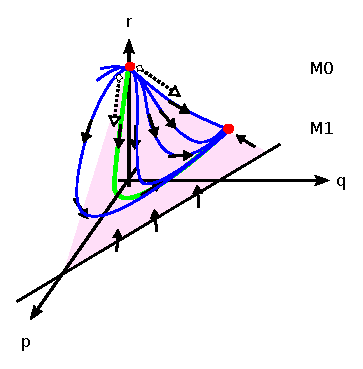
\includegraphics[width=3cm]{h_func.eps}
%   } \quad \quad \quad
%   \subfigure[Required behavior]{
%     \psfrag{p}{\scriptsize$p$}
%     \psfrag{q}{\scriptsize$q$}
%     \psfrag{M0}{\scriptsize$M_0$}
%     \psfrag{X01}{\scriptsize$\vec{X}_{02}$}
%     \psfrag{X02}{\scriptsize$\vec{X}_{01}$}
%     \includegraphics[width=3cm]{neighborhood.eps}
%   }
%   \caption{Conjectured heteroclinic orbit.}
% \end{figure}
% \end{frame}

\begin{frame}
 \setstretch{1.5}
 \frametitle{Heteroclinic for the inviscid problem: $n=0$}
 {\bf Lemma 1.} There is the most rapidly escaping orbit $\phi^\star(\eta)$ that escapes the region $A$ in the first quadrant satisfying the estimate
 $e^{-2\eta}\Big(\phi^\star(\eta)- M_0\Big) \rightarrow \kappa\vec{X}_{01}$, as $\eta \rightarrow -\infty$.
 \begin{figure}
  \centering
%   \psfrag{X01}{\scriptsize$X_{02}$}
%   \psfrag{X02}{\scriptsize$X_{01}$}
% %   \psfrag{A}{$A$}
%   \psfrag{T}{\scriptsize $B$}
% %   \psfrag{x0}{\scriptsize $M_0$}
% %   \psfrag{x1}{\scriptsize $M_1$}
% %   \psfrag{r0}{\scriptsize $\hat{r}(p,q,s,0)=r_0$}
% %   \psfrag{r1}{\scriptsize $\hat{r}(p,q,s,0)=r_1$}
%   \psfrag{p}{\scriptsize $p$}%=\frac{\gamma}{\sigma}$}
%   \psfrag{q}{\scriptsize~~~$q$}%=n\frac{v}{\sigma}$}
%   \psfrag{s}{\scriptsize $s-\frac{1+m}{1+\alpha}$}%=n\frac{v}{\sigma}$}
% %   \subfigure[Affine level sets $\hat{r}(p,q,s)=R$ in $pqs$-space]{
% %   \psfrag{r}{\scriptsize$r$}%=\big(\sigma\gamma^{(1-n)}\big)^{\frac{1}{n}}$}
%   \psfrag{CC}{\scriptsize\hskip 5pt$\frac{\alpha-m}{\lambda(1+\alpha)}\big(-\frac{1}{\lambda},a\big)$}
  \includegraphics[width=5cm]{geom0.eps} \label{fig:flow0}  
%   
%   
%     \psfrag{p}{\scriptsize$p$}
%     \psfrag{q}{\scriptsize$q$}
%     \psfrag{X01}{\scriptsize$\vec{X}_{01}$}
%     \psfrag{X02}{\scriptsize$\vec{X}_{02}$}
%     \psfrag{T}{\scriptsize $~~B$}
%     \psfrag{3}{}
%     \subfigure{\includegraphics[width=4cm]{geom1.eps} } \quad \quad \quad
%     \subfigure{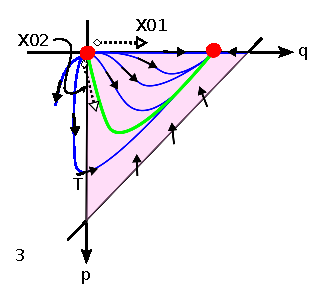
\includegraphics[width=3cm]{pqplane.eps}}
% %     \includegraphics[width=5cm]{.eps}
 \end{figure}
 {\scriptsize
 {\bf \it Proof.}
  $A$ is a 2-dimensional compact negatively invariant set. There is no limit cycle in $A$. By Poincar\'e-Bendixson Theorem, $\alpha$-limit point of every orbit in $A$ is $M_0$. Similar arguments for $T$.
 }
\end{frame}

\begin{frame}
 \setstretch{1.5}
 \frametitle{Heteroclinic for the inviscid problem: $n=0$}
 {\bf Lemma 2.} $W^s(M_1) = \Phi_{-t_0}\big(W^s_{loc}(M_1)\big)$, the time $-t_0$ image of $W^s_{loc}(M_1)$ for large enough $t_0$, is the three dimensional set and contains an orbit point of $\phi^\star(\eta)$ as an interior point.
   \begin{figure}
  \centering
    \psfrag{p}{\scriptsize$p$}
    \psfrag{q}{\scriptsize$q$}
    \psfrag{s}{\scriptsize$s-\frac{1+m}{1+\alpha}$}
    \psfrag{X01}{\hskip -7pt\scriptsize$\vec{X}_{01}$}
    \includegraphics[width=3.3cm]{transversal3.eps}
    \caption{3-dim stable manifold}
 \end{figure}
 \vskip -15pt
 {\scriptsize
 {\bf \it Proof.}
  %$B$ is a 2-dimensional compact positively invariant set. Similarly as before, $\omega$-limit point of every orbit in $B\setminus M_0$ is $M_1$. 
  $W^s(M_1) = \Phi_{-t_0}\big(W^s_{loc}(M_1)\big)$, the image of the diffeomorphism $\Phi{-t_0}$, is a three dimensional set and contains an orbit point of $\phi^\star(\eta)$ in its interior because of Lemma 1.
 }
\end{frame}


% \begin{frame}
%  \setstretch{1.5}
%  \frametitle{Heteroclinic for the inviscid problem: $n=0$}
%  {\bf Lemma 2.} The trapezoid except $s$-axis, $K\setminus \{s-axis\}\subset W^s(M_1)$.
%   \begin{figure}
%   \centering
%     \psfrag{p}{\scriptsize$p$}
%     \psfrag{q}{\scriptsize$q$}
%     \psfrag{B}{\scriptsize$B$}
%     \psfrag{K}{\scriptsize$K$}
%     \psfrag{s}{\scriptsize$s-\frac{1+m}{1+\alpha}$}
%     \psfrag{x0}{\scriptsize $M_0$}
%     \psfrag{x1}{\hskip -3pt\scriptsize $M_1$}
%     \psfrag{X01}{\scriptsize$\vec{X}_{01}$}
%     \psfrag{X02}{\scriptsize$\vec{X}_{02}$}
%     \includegraphics[width=3.5cm]{flow0pqs.eps}
%     %\quad \quad {\scriptsize Note that $ \dot{s} = -\frac{1+\alpha}{\lambda}\hat{r}(p,q,s)s\Big(s-\frac{1+m}{1+\alpha}\Big)$, and $\hat{r}(p,q,s)\ge\delta>0.$}
%  \end{figure}
%  {\scriptsize
%  {\bf \it Proof.}
%   $B$ is a 2-dimensional compact positively invariant set. Similarly as before, $\omega$-limit point of every orbit in $B\setminus M_0$ is $M_1$. In particular, the set $B$ is an {\blue positively invariant set with hyperbolic splitting} of tangent bundle. By Fenichel's Expanding Fiber Theorem, there is a 3-dimensinal manifold that approaches to $B$. Every orbit in $K\setminus \{$s$-axis\}$ touches this $3$-dimensional manifold in a finite time.
%  }
% \end{frame}

\begin{frame}
 \setstretch{1.3}
 \frametitle{Heteroclinic for the inviscid problem: $n=0$}
 {\bf Corollay 3.} The most rapidly escaping orbit $\phi^\star(\eta)\subset W^u(M_0)$ intersects $W^s(M_1)$ transversally.
   \begin{figure}
  \centering
    \psfrag{p}{\scriptsize$p$}
    \psfrag{q}{\scriptsize$q$}
    \psfrag{B}{\scriptsize$B$}
    \psfrag{K}{\scriptsize$K$}
    \psfrag{s}{\scriptsize$s-\frac{1+m}{1+\alpha}$}
    \psfrag{x0}{\scriptsize $M_0$}
    \psfrag{x1}{\hskip -3pt\scriptsize $M_1$}
    \psfrag{X01}{\scriptsize$\vec{X}_{01}$}
    \psfrag{X02}{\scriptsize$\vec{X}_{02}$}
    \subfigure[$\Phi_{-t_0}\big(W^s_{loc}(M_1)\big)$] {\includegraphics[width=3cm]{transversal.eps} } \quad \quad \quad
    \subfigure[schematic sketch]{\includegraphics[width=3cm]{flow0pqs.eps}}
    %\quad \quad {\scriptsize Note that $ \dot{s} = -\frac{1+\alpha}{\lambda}\hat{r}(p,q,s)s\Big(s-\frac{1+m}{1+\alpha}\Big)$, and $\hat{r}(p,q,s)\ge\delta>0.$}
 \end{figure}
 
 \vskip -8pt
%\vfill
{\bf Remark.} The invariant manifolds of {\blue $r=\hat{r}(p,q,s)$, $M_0$, $M_1$, the most rapidly escaping orbit from $M_0$, $W^s(M_1)$} are all stable under $C^1$-perturbation of the vector fields; transversal intersection is stable under $C^1$-perturbation. 
\end{frame}

\begin{frame}
\setstretch{1.5}
  {\bf Theorem.} Let $\Lambda$ be a domain of the tuple $(\lambda,\alpha,m,n)\in\mathbb{R}^4$ defined by %.Suppose the three parameters $(\lambda,m,n)$ are such that
  {\scriptsize
 \begin{align*}
  \alpha>0\quad&\text{(thermal softening)},\\
  m>-1 \quad&\text{(strain softening/hardening)}, \\%\label{eq:a1}\\
  n>0 \quad&\text{(rate sensitivity)},\\ %\label{eq:a2}\\
  -\alpha+m+n<0 \quad&\text{(net softening)}, \\%\label{eq:a3}\\
  0< \lambda < \frac{2(\alpha-m-n)}{1+m+n}\left(\frac{1+m}{1+m+n}\right) \quad&\text{(rate bound)}. %\label{eq:a4}
\end{align*}}
 For each $(\lambda,\alpha,m,0) \in \Lambda$, there is $n_0( \lambda,\alpha,m)$ such that for $n \in [0, n_0)$, $(\lambda,\alpha,m,n) \in \Lambda$ and the system $(*)^{\lambda,\alpha,m,n}$ admits a heteroclinic orbit joining equilibrium $M_0^{\lambda,\alpha,m,n}$ to equilibrium $M_1^{\lambda,\alpha,m,n}$ with property that
    \begin{align*}% \label{eq:estimate}
        &\chi(\eta) \rightarrow M_1 \quad \text{as $\eta \rightarrow \infty$ and} \\
        &e^{2\eta}\big(\chi(\eta) - M_0\big) \rightarrow \kappa X_{01} \quad \text{as $\eta \rightarrow -\infty$ for some $\kappa\ne0$}.
    \end{align*}
% \end{theorem}
\end{frame}








% 
% \begin{frame}
%  \begin{theorem} \label{thm1}
% Let $\alpha>0$, $m>-1$, $-\alpha+m>0$ and $0<\lambda< \frac{2(\alpha-m)}{1+m}$. For the pair $(\lambda,\alpha,m)$, there exists $n_0$ such that for all $n \in [0,n_0)$
% \begin{enumerate}
%     \item[(i)] the tuple $(\lambda,\alpha,m,n)$ satisfies  $0< \lambda < \frac{2(\alpha-m-n)}{1+m+n}\left(\frac{1+m}{1+m+n}\right)$.
%     \item[(ii)] $(p,q,r,s)$-system with parameters $(\lambda,\alpha,m,n)$ admits a heteroclinic orbit $\chi(\eta)$ such that
%     \begin{align*}% \label{eq:estimate}
%         &\chi(\eta) \rightarrow M_1 \quad \text{as $\eta \rightarrow \infty$ and} \\
%         &e^{2\eta}\big(\chi(\eta) - M_0\big) \rightarrow \kappa X_{01} \quad \text{as $\eta \rightarrow -\infty$ for some $\kappa\ne0$}.
%     \end{align*}
% \end{enumerate}
% \end{theorem}
% \end{frame}

% \begin{frame}
% \setstretch{1.5}
% Let $(\alpha,m,n)$ be the given material property.
% 
% In summary, %for each $\big(\Gamma(0),U(0)\big)$ such that ({\scriptsize two of $\Gamma(0),U(0),\lambda$ fix the rest})
% % \begin{equation*}
% %  \frac{2(1+\alpha) -n}{D} < \frac{U(0)}{\Gamma(0)} < \frac{2(1+\alpha)}{1+m+n} -\frac{n}{D}\left( \frac{4(1+\alpha)(\alpha-m-n)}{(1+m+n)^2} +1\right),
% % \end{equation*}
% if $n$ is sufficiently small, then we have the solution of following form.
% \begin{equation*} %\label{intro-sols}
% \begin{aligned}
%  \bg(t,x) &= (t+1)^a\Gamma\big((t+1)^\lambda x\big), \\
%  \bv(t,x) &= (t+1)^b V\big((t+1)^\lambda x\big), \\
%  \bth(t,x) &= (t+1)^c\Theta\big((t+1)^\lambda x\big),\\
%  \bs(t,x) &= (t+1)^d\Sigma\big((t+1)^\lambda x\big), \\
%  \bu(t,x) &= (t+1)^{a-1}U\big((t+1)^\lambda x\big),
% \end{aligned}
% \end{equation*}
% $$ \bv(t,x) \rightarrow (t+1)^b V_\infty, \: \text{as $x \rightarrow \infty$}; \quad \bv(t,x) \rightarrow -(t+1)^b V_\infty, \: \text{as $x \rightarrow -\infty$}.$$
% \vfill
% %Note that the $\big(\bG,\bV,\bS,\bU\big)$ coincide with the initial nonuniformities of $\big(\gamma,v,\sigma,u\big)$ at $t=0$. 
% %\vfill
% \end{frame}      



\begin{frame}
 \setstretch{1.3}
 \frametitle{Original field variables at various instances of time.}%  $\lambda=10$, $n=0.05$, $m=-1$, $\alpha=0$.}
 \begin{figure}
  \centering
  \subfigure[strain] {
    \includegraphics[width=3.5cm]{strain_log.eps}
  }
  \quad
  \subfigure[strain rate] {
    \includegraphics[width=3.5cm]{strain_rate_log.eps}
  }
  \\
  \subfigure[velocity] {
    \includegraphics[width=3.5cm]{velocity.eps}
  }
  \quad
  \subfigure[stress] {
    \includegraphics[width=3.5cm]{stress_log.eps}
  } %\caption{Original field variables at various instances of time.  $\lambda=10$, $n=0.05$, $m=1$.}
 \end{figure}
\end{frame}

\begin{frame}
 \center
 \vfill
 
 {\bf \huge \blue  Thank you very much.}
 
 \vfill
\end{frame}

\begin{frame}
 \setstretch{1.3}
 At $n=0$, rich structures are explicitly available; planar dynamical system theory is enough to furnish the existence of the heteroclinic.
 \begin{figure}
  \centering
  \setcounter{subfigure}{0}
%   \psfrag{x0}{\tiny $M_0$}
%   \psfrag{x1}{\tiny $M_1$} 
%   \psfrag{M_0}{\tiny $M_0$}
%   \psfrag{M_1}{\tiny $M_1$}   
  \psfrag{p}{\tiny $p$}
  \psfrag{q}{\tiny $q$}
  \psfrag{s}{\tiny \hskip -1em $s-\tfrac{1+m}{1+\alpha}$}
  \psfrag{r}{\tiny $r$}
  \psfrag{K}{\tiny \hskip -1em $N_0$}
    \includegraphics[width=2.5cm]{flow0pqs.eps}
  \quad \quad
    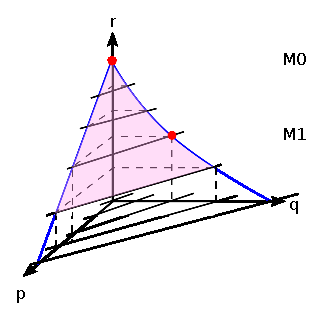
\includegraphics[width=2.5cm]{h_n0func.eps}
  \quad \quad
  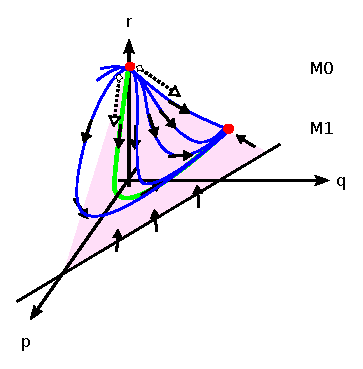
\includegraphics[width=2.5cm]{h_func.eps}
 \end{figure}
\vskip -2em
{\tiny
 \begin{align*}
 \dot{p} &=p\Big(\frac{1}{\lambda}(r-a) + 2- \lambda p r -q\Big),\\
 \dot{q} &=q\Big(1 -\lambda p r -q\Big) + b p r,\\
 n\dot{r} &=r\Big(\frac{\alpha-m-n}{\lambda(1+\alpha)}(r-a) + \lambda pr + q +\frac{\alpha}{\lambda}\Big(r\big(s- \frac{1+m+n}{1+\alpha}\big) + \frac{n}{(1+\alpha)}\Big)\Big),\\
 \dot{s} &=s\Big(\frac{\alpha-m-n}{\lambda(1+\alpha)}(r-a) + \lambda pr + q - \frac{1}{\lambda}\Big(r\big(s- \frac{1+m+n}{1+\alpha}\big) + \frac{n}{(1+\alpha)}\Big)\Big),
 \end{align*}
 }
\vskip -2em
 We want to reproduce the orbit via abstract invariant manifold theory.
\end{frame}

\begin{frame}
\frametitle{Heteroclinic orbit}
 \begin{figure}
  \psfrag{p}{\scriptsize $p$}
  \psfrag{q}{\scriptsize $q$}
  \psfrag{s}{\scriptsize \hskip -2em $s-\tfrac{1+m}{1+\alpha}$}
  \psfrag{N2}{\scriptsize $N_2$}
  \psfrag{F2}{\tiny normal foliations}% $\mathcal{F}(N_2)$}
  \psfrag{M0}{\tiny $M_0$}
  \psfrag{M1}{\tiny $M_1$}
  \psfrag{F0}{}%{\tiny \hskip -10em $M_0\xhookrightarrow{} N_2\xhookrightarrow{} \underbrace{N_2\oplus \mathcal{F}(N_2)}_{\triangleq N_1} $}
  \psfrag{F1}{}%{\tiny $M_1\xhookrightarrow{} W^s(M_1)\xhookrightarrow{} W^s(M_1)\oplus \mathcal{F}(N_0)$}
  \includegraphics[width=7cm,height=3.5cm]{Hetero_Foliation.eps}
%   \caption{Heteroclinic connecting $M_0$ to $M_1$ when $n=0$.}
 \end{figure}
{ \tiny
(In fact, the complete picture around $M_0$ and $M_1$ are characterized dimension by dimension)
\begin{align*}
 B_\delta(M_0): ~~ M_0&\xhookrightarrow{} N_2\xhookrightarrow{} \underbrace{N_2\oplus \mathcal{F}(N_2)}_{\triangleq N_1} &&\xhookrightarrow{} \underbrace{N_2\oplus \mathcal{F}(N_2)\oplus \mathcal{F}(N_1)}_{\text{open in } N_0} &&\xhookrightarrow{} N_2\oplus \mathcal{F}(N_2)\oplus \mathcal{F}(N_1) \oplus \mathcal{F}(N_0)\subset \mathbb{R}^4\\
 B_\delta(M_1): ~~ M_1& & &\xhookrightarrow{} \overbrace{W^s(M_1)}^{\text{open in } N_0}&&\xhookrightarrow{} W^s(M_1)\oplus \mathcal{F}(N_0)\subset \mathbb{R}^4
\end{align*}
}

% $\mathcal{F}(N_2)$ and $W^{s}(M_1)$ are effectively chosen to characterize the orbit:
\begin{proposition}
 At $n=0$, the finite time extensions of $\mathcal{F}(N_2;M_0)$ and $W^{s}(M_1)$ intersect transversally.
\end{proposition} 
 
\end{frame}


\begin{frame}
 \setstretch{1.3}
 \frametitle{Heteroclinic orbit}
{\scriptsize 
 Fenichel Theorem: Provided $M_0, N_0, \cdots , N_2$ {\blue normally hyperbolic}, $M_{0n}$, $N_{0n}, \cdots$ and all their local foliations $\mathcal{F}(M_{0n})$, $\mathcal{F}(N_{0n}), \cdots$ {\blue exists} as a $C^r$- families in $n$, sufficiently small.
} 

\begin{corollary}
 For $n>0$ sufficiently small, $\mathcal{F}(N_2;M_0(n))$ and $W^{s}(M_1(n))$ again intersect transversally, forming the heteroclinic orbit.
\end{corollary}

\end{frame}

\begin{frame}
 \setstretch{1.2}
 \frametitle{Numerical computation of the heteroclinic}%Continuation method '89 Doedel, Friedman}
 Problem of detecting a {\red saddle-saddle} connection:
 \begin{figure}
  \includegraphics[width=4cm,height=2.7cm]{saddle_saddle.eps}
  \caption{\scriptsize Any time integrator would suffer the instability.}
 \end{figure}
 {\scriptsize
 Recall that
 \begin{align*}
 M_0 \quad &\text{has (3 unstable, 1 stable) dimensions},\\             
 M_1 \quad &\text{has (1 unstable, 3 stable) dimensions.}
 \end{align*}
 }
 Goal: To capture {\red 1-dim curve} $\xhookrightarrow{}$ 2-dim surface $\xhookrightarrow{}\mathbb{R}^4$ that is the intersection of the unstable and stable manifold of $M_0$ and $M_1$ respectively.
 
\end{frame}

\begin{frame}
 \setstretch{1.2}
 \frametitle{Continuation method '89 Doedel, Friedman}
 \begin{figure}
  \psfrag{T}{}%\tiny $t\in[-T,T]$}
  \psfrag{e0}{\tiny $\epsilon_0 \nu_0,$}
  \psfrag{nu0}{\tiny $\nu_0 \in \mathbb{S}^{n_u - 1}$}
  \psfrag{e1}{\tiny $\epsilon_1 \nu_1$,}
  \psfrag{nu1}{\tiny $\nu_1 \in \mathbb{S}^{n_s - 1}$}  
  \includegraphics[width=6cm,height=3cm]{autoform.eps}
 \end{figure}
 {\scriptsize
 Suppose $x^*(t)$ is a heteroclinic orbit. Pick $T$ large and $\epsilon_0^*$, $\nu_0^*$, $\epsilon_1^*$, and $\nu_1^*$ so that
 $$\pi_u\big(x^*(-T)-M_0\big) = \epsilon_0^*\nu_0^*, \quad\pi_s\big(x^*(T)-M_1\big) = \epsilon_1^*\nu_1^*.$$
 Then $U^*= (x^*(t),P^*) \in C^1(-\infty,\infty) \times \mathbb{R}^{n_p}$, $P^*=(\alpha,m,n,\lambda, \epsilon_0^*,\nu_0^*,\epsilon_1^*,\nu_1^*)$ is a solution of following algebro-differential nonlinear system
 \begin{align*}
  &x'(t) - f(x,P) =0, \quad t\in (-\infty,\infty),\\
  &\pi_u\big(x(-T)-M_0\big) = \epsilon_0\nu_0, \quad\pi_s\big(x(T)-M_1\big) = \epsilon_1\nu_1.
 \end{align*}
 }
\end{frame}

\begin{frame}
 \setstretch{1.2}
 {\scriptsize
 Seemingly sounder formulation is possible: An algebro-differential system on $V= (y(t),P) \in C^1(-\infty,\infty) \times \mathbb{R}^{n_p}$, 
 
 $x(t) = y(t) +\chi^*(t)$, for some fixed smooth $\chi^*(t)$, i.e., %where $\chi^*(t) = M_0$, $t\in(-\infty,-T-\delta)$ and $\chi^*(t) = M_1$, $t\in(T+\delta,\infty)$.
 \begin{equation*}(*)\left\{
 \begin{aligned}
  &y'(t) +\chi^{*\prime}(t) - f(y+\chi^*,P) =0, \quad t\in (-\infty,\infty),\\
  &\pi_u~y(-T) = \epsilon_0\nu_0, \quad \pi_s~y(T) = \epsilon_1\nu_1.
 \end{aligned}\right.
 \end{equation*}
 Let us write above $F(V) = 0$. We see $V^*=\big(y^* (= x^*-\chi^*),P^*)$ solves this. 
 \pause
 We pose an approximation problem to $(*)$:
 \begin{equation*}(*)_{app}\left\{
 \begin{aligned}
  &y'(t) +\chi^{*\prime}(t) - f(y+\chi^*,P) =0, \quad t\in (-T,T),\\
  &y(t), t\in (-\infty,-T)\cup (T,\infty): ~~ \text{evolution from $-T$ and $T$ {\blue Linearly},}\\
  &y(-T) = \epsilon_0\nu_0, \quad y(T) = \epsilon_1\nu_1.
 \end{aligned}\right.
 \end{equation*}
 Suppose $F(V)$ has the nontrivial kernel in the nhd of $P^*$ of the form $y(P)$, $F\big(y(P),P\big)=0$.
 
 Then we expect solvability of $(*)_{app}$ as well in the nhd of $P^*$. The software \texttt{AUTO} (Doedel, Friedman) implements this program.
 } 
\end{frame}

\begin{frame}
 \setstretch{1.2}
  \begin{figure}
  \centering
  \setcounter{subfigure}{0}
  \subfigure[$(\alpha,m,\lambda)$ continuation] {
    \includegraphics[width=3.5cm]{QRcont.eps}
  }
  \quad
  \subfigure[$(\nu_0,\nu_1)$ continuation] {
    \includegraphics[width=3.5cm]{nu0nu1cont.eps}
  }
  \\
  \subfigure[Heteroclinic orbit] {
    \includegraphics[width=3.5cm]{hetero.eps}
  }
  \caption{\scriptsize Heteroclinic at $\alpha = 7.66$, $m=2.58$, $n=0.1$, $\lambda=2.32$, $\eps_0=3.7e-3$, $\nu_0=X_{01}$, $\eps_1=2.7e-4$.}
 \end{figure}

\end{frame}



\end{document}


\begin{frame}
 \setstretch{1.2}
 \frametitle{Hadamard Instability}
 
 \begin{minipage}{0.35\linewidth}
  \begin{figure}
    \center
    \psfrag{stress}{\scriptsize \hskip -3em stress $\sigma$}
    \psfrag{strain}{\scriptsize strain $\gamma$}
    \psfrag{phi}{\scriptsize  $\varphi^{'}( \gamma ) < 0$}% = \frac{1}{\gamma}$}
    \includegraphics[width=2.8cm]{phi.eps}
    \caption{Plastic response}
  \end{figure}
 \end{minipage}
 \begin{minipage}{0.6\linewidth}
 \begin{itemize}
  \item   When material is under {\blue plastic} deformation, material softens as strain increases and {\blue instability} takes place. 
  \item Observe that the model with $n=0$
  \begin{align*}
     \begin{aligned}
          \partial_t v &= \partial_x\Big(\varphi(\gamma)\Big), \quad \varphi^\prime <0,\\
          \partial_t \gamma &= \partial_x v,
     \end{aligned} 
  \end{align*}
  loses hyperbolicity. 
 \end{itemize}
 \end{minipage}
 \vfill
 IVP of elliptic system indicates the catastrophic growth of oscillations, the {\blue Hadamard Instability}.
  \vfill
\end{frame}



\begin{frame}
 \frametitle{Viscosity regularizes the problem}
 \setstretch{1.5}
 Parametric study for the form of $\sigma = \varphi(\gamma)\gamma_t^n = \gamma^{-m}\gamma_t^n$ shows that \vfill
 \begin{itemize}
  \item $-m+n>0$ 
  
  {\footnotesize Tzavaras (1992)} : USS is non-linearly stable.
  \item $n=0$ 
  
  Hadamard Instability: System loses hyperbolicity forming ivp of an elliptic system.
  \item $n\ne0$, $-m+n<0$ : 
 \end{itemize}
 \vfill
\end{frame}

\begin{frame}
 \setstretch{1.5}
 \frametitle{Hadamard instability vs. non-linearity.}
 The model
\begin{equation*} %\label{system0}
    \begin{aligned}
      \partial_t v &= \partial_x\Big(\varphi(\gamma)\, v_x^n\Big), \\
      \partial_t \gamma &= \partial_x v
    \end{aligned}
 \end{equation*}
 is a paradigm capturing the bare essentials of that coherent localization in the rate-dependent shear deformation.% in the simplest setting.
 \vfill
 {\blue Question.}
 
 Out of the {\red competition} between the {\blue Hadamard Instability} and the {\blue non-linearity} of rate-dependence, can the model exhibit the coherent localization?
 \vfill
\end{frame}


\begin{frame}
 \setstretch{1.5}
 \frametitle{Stability problem of USS, $m=1$, $-1+n<0$}
 Because this benchmark solution is {\it time-dependent}, even linearized study suffers from the {\it non-autonomous} issues, i.e., linearized equations have time-dependent coefficients. However, when $m=1$, 
 $$\sigma(\gamma,\gamma_t) = \varphi(\gamma)\gamma_t = \gamma^{-1}\gamma_t = \frac{\gamma_t}{\gamma},$$
 the relatively perturbed fields $(\Gamma,\Sigma,U)$ can be introduced\footnote[frame]{Molinari and Clifton(1987)}
\begin{equation*}
% \label{intro-rescale}
\begin{aligned}
 \Gamma(x, \tau(t)) &= \frac{\gamma(x,t)}{\gamma_s(t)}\, , \quad \Sigma(x, \tau(t))= \frac{\sigma(x,t) }{\sigma_s(t)}\\
 U (x,\tau(t)) &= u (x,t) :=v_x (x,t)\, ,  \quad  \mbox{where} \quad \tau(t) = \log(1+ \frac{t}{\gamma_0}) \, ,
\end{aligned}
\end{equation*}
\end{frame}

\begin{frame}
  \setstretch{1.2}
\frametitle{Stability problem of USS, $m=1$, $-1+n<0$}
and the problem of stability of uniform shearing solution is transformed into the problem
of stability of the {\blue equilibrium $( \bar U , \bar \Gamma ) = (1,1)$} for the {\blue nonlinear} but  {\blue autonomous} parabolic system\footnote[frame]{Katsaounis and Tzavaras(2009)} 
\begin{align*}
 U_\tau = \Sigma_{xx} =\bigg( \frac{U^n}{\Gamma}\bigg)_{xx} \, , \quad  \Gamma_\tau = U - \Gamma \, .
%  \label{intro-redsys}
\end{align*} 

The heuristic argument can be developed that the second equation {relaxes} to the equilibrium manifold $\{ U = \Gamma \}$ and the stability is determined by the {\blue effective equation}
\begin{equation*}
U_\tau = \Sigma_{xx} =\big(  U^{n-1} \big)_{xx} \, .
\end{equation*}
The latter is {backward parabolic} for $n < 1$, what suggests {\it instability} in this regime $n < 1$.
\end{frame}

\begin{frame}
  \setstretch{1.5}
   \frametitle{Turing instability of Linearized problem.}
   Another understanding can be gained from the {\blue linear stability}.  Linearized system around $( \bar U , \bar \Gamma ) = (1,1)$
  \begin{equation*}
% \label{intro-linp}
\begin{aligned}
{\tilde{U}}_\tau &= n \tilde{U}_{xx}  - \tilde\Gamma_{xx}, 
\\
{ \tilde\Gamma }_\tau &= \tilde{U} - \tilde\Gamma  
\end{aligned}
\end{equation*}
have {\blue growing modes}. From Fourier series analysis,

\vfill
   {\bf Case $n=0$} (Hadamard Instability) : There are positive eigenvalues $\lambda_j^+$ for each $j\ge0$ and $\lambda_j^+ \rightarrow \infty$ as $j \rightarrow \infty$.
\end{frame}

\begin{frame}
  \setstretch{1.5}
   \frametitle{Turing instability of Linearized problem.}
   {\bf Case $0<n<1$} {\red (Turing instability)} : 
   \begin{enumerate}
    \item $\lambda^+_j$ is increasing in $j$,
    \item $\lambda^+_j < \frac{1-n}{n}$,
    \item $\lambda^+_j \rightarrow \frac{1-n}{n}$ \quad as\quad $j \rightarrow \infty$.
  \end{enumerate}
   Observe the Turing instability in the coefficient matrix,
\begin{align*}
  \begin{pmatrix}
  \hat{U}_j(t) \\
  \hat{\Gamma}_j(t)
 \end{pmatrix}^\prime &=\left[   
 \begin{pmatrix}
  - nj^2\pi^2 & j^2\pi^2 \\
  1 & - 1
 \end{pmatrix}\right]\begin{pmatrix}
  \hat{U}_j(t) \\
  \hat{\Gamma}_j(t)
 \end{pmatrix} \\&=
 \left[   
 \begin{pmatrix}
  - nj^2\pi^2 & 0 \\
  1 & 0
 \end{pmatrix} +
  \begin{pmatrix}
  0 & j^2\pi^2 \\
  0 & - 1
 \end{pmatrix}\right]\begin{pmatrix}
  \hat{U}_j(t) \\
  \hat{\Gamma}_j(t)
 \end{pmatrix}.
\end{align*}

\end{frame}







\begin{frame}
 \frametitle{A family of focusing self-similar solutions}
 \setstretch{1.5}
   {The objective of this talk} is to give an ample demonstration of the onset of localizing instability by constructing {\blue a family of {\red focusing} solutions} for the range of parameters $-m+n<0$, $n\ll1$,
\begin{equation*}
 \begin{aligned}
% v(x,t) &= \Big(1 + \frac{t}{ \gamma_0 } \Big)^{ \frac{ \lambda n}{2-n} } \;\bV\bigg(x\Big(1 + \frac{t}{ \gamma_0 } \Big)^{\lambda}\bigg),\\
 \gamma(x,t) &= (1 + t)^{ \frac{2-n}{1+m-n}+ \frac{ 2 }{1+m-n}\lambda } \;\bG\Big(x(1 + t)^{\lambda}\Big), \\
 v(x,t) &= (1 + t)^{ \frac{1-m}{1+m-n}+ \frac{ 1-m+n }{1+m-n}\lambda } \;\bV\Big(x(1 + t)^{\lambda}\Big), \\
 \sigma(x,t) &= (1 + t)^{ -\frac{2m-n}{1+m-n} - \frac{ m-n }{1+m-n}\lambda } \;\bS\Big(x(1 + t)^{\lambda}\Big), \\
 u(x,t) &=   v_x (x,t)  = (1 + t)^{\frac{1-m}{1+m-n}+ \frac{ 2 }{1+m-n}\lambda} \;\bU\Big(x(1 + t)^{\lambda}\Big), \\
 \end{aligned} %\label{intro-ss}
\end{equation*}
where $x(1 + t)^{\lambda}=\xi$ is the similarity variable and $\lambda>0$ accounts for the rate of focusing.
\end{frame}

\begin{frame}
 \frametitle{Coherent localization}
 \setstretch{1.5}
   \setcounter{subfigure}{0}
   \begin{figure}
	\subfigure[strain in log scale]{
	  \includegraphics[width=4.5cm]{strain_log.eps} %\vskip -5pt
	}
	\quad \quad
	\subfigure[velocity]{
	  \includegraphics[width=4.5cm]{velocity.eps} %\vskip -5pt
	}
   \caption{Emergence of coherent localization: shear bands.}
  \end{figure}
\end{frame}




\begin{frame}
 \frametitle{Scale invariance and self-similar solutions}
 \setstretch{1.2} 
 We return to the system .
 \begin{align*}
  \begin{aligned}
    v_t &= \Big(\varphi(\gamma)\gamma_t^n\Big)_x = \Big(\gamma^{-m}\,\gamma_t^n\Big)_x, \\
    \gamma_t &= v_x
  \end{aligned}
 \end{align*}
 with $-m+n<0, \, n\ne0$. We begin with investigating the scale invariance.
 
\vfill
% We begin with investigating the {\blue family of scale invariances} of the system. 
Define $(\gamma_\rho$, $v_\rho)$ for given $(\gamma,v)$ such that
\begin{align*}
 \gamma_\rho(t,x) &= \rho^a \gamma(\rho^{-1}t, \rho^\lambda x), \\
 v_\rho(t,x) &= \rho^b v(\rho^{-1}t, \rho^\lambda x). \qquad \text{ \blue \footnotesize($\lambda>0$ for focusing type.)}
%  &s=\rho^{-1}t, \quad
%  y=\rho^ \lambda x, \qquad \text{ \blue \footnotesize($\lambda>0$ for focusing type.)}
\end{align*}
A family of the exponents $a$ and $b$ making system invariant are 
\begin{equation*} %\label{eq:s_inv}
 a^{\lambda,m,n}= \frac{2-n}{1+m-n} + \frac{2}{1+m-n}\lambda, \quad b^{\lambda,m,n}= \frac{1-m}{1+m-n} + \frac{1-m+n}{1+m-n} \lambda.
\end{equation*}
\end{frame}

\begin{frame}
 \frametitle{Scale invariance and self-similar solutions}
 \setstretch{1.2} 
 Motivated from scale invariances, consider {\blue a family of focusing self-similar solutions}
% Now, we consider a  parametrized by $\lambda$ and by given $m$ and $n$ such that
\begin{align*}
 \bar{ \gamma }(t,x) &= t^a \bar{ \gamma}(1, t^ \lambda x)=t^a\bG(t^ \lambda x),\\
 \bar{v}(t,x)&=t^b \bar{ v}(1, t^ \lambda x)=t^b\bV(t^ \lambda x)
\end{align*}
and {\blue $\xi=t^ \lambda x$} is the {\blue similarity variable}. 

\vfill
Substitution of this form induces a system of ordinary differential equations
\begin{equation*} %\label{eq:sseqns}
 \begin{split}
 a^{\lambda,m,n}\bG + \lambda \xi \bG_\xi &= \bV_\xi,\\
 b^{\lambda,m,n}\bV + \lambda \xi \bV_\xi &= \big(\bG^{-m}\bV_\xi^n\big)_\xi.
 \end{split}
\end{equation*}
\end{frame}

\begin{frame}
 \frametitle{Self-similar equations with singularity at $\xi=0$}
 \setstretch{1.3} 
%  Solutions for a given $m$ and $n$ that localize in a self-similar way at localizing rate $\lambda$ will be attained by achieving solutions of system.
 The system
\begin{equation*} 
 \begin{split}
 a^{\lambda,m,n}\bG + \lambda \xi \bG_\xi &= \bV_\xi,\\
 b^{\lambda,m,n}\bV + \lambda \xi \bV_\xi &= \big(\bG^{-m}\bV_\xi^n\big)_\xi.
 \end{split}
\end{equation*}
has a {\blue singularity} at $\xi=0$ ({\footnotesize Note $\xi$ in front of $\bG_\xi$ the highest derivative of $\bG$}). 
\vfill
\begin{enumerate}
 \item For such a singular system, case-by-case study determines whether or not it has solutions. 
 \item For our case, this system is successfully {\red de-singularized} and is formulated into an {\red autonomous system }of three first-order equations. 
 \item The solution will be attained as a suitable {\red heteroclinic connection} of this dynamical system.
\end{enumerate}
\end{frame}

\begin{frame}
 \frametitle{Construction of the family of focusing self-similar solutions}
 \setstretch{1.5}
 We will carry out several steps ({\footnotesize Katsaounis, Olivier and Tzavaras (2014)}) :
 \begin{enumerate}
  \item {\blue De-singularize} of the singular self-similar equations to obtain the autonomous system.
  \item {\blue Identify  equilibrium} points and their local eigen-structures respectively of the dynamical system.
  \item Inspect physically admissible {\blue asymptotic behavior as $\eta \rightarrow\pm\infty$} that eventually provides the {\blue characterization} of the unique heteroclinic connection in phase space.
  \item Construct the target orbit via {\blue geometric singular perturbation theory + Poincar\'e-Bendixson.}
 \end{enumerate}
\end{frame}

\begin{frame}
 \frametitle{De-singularization}
 \setstretch{1.5}
 We look for $\bG$ that is {\blue even} and $\bV$ that is {\blue odd} and restrict the domain to $\xi\ge0$ with {\red regularity conditions}
 \begin{equation*} %\label{eq:continuity}
 \frac{d}{d\xi}\bG(0)=\bV(0)=0.
 \end{equation*}
New scaled variables {\red $(\tg,\tv,\tu,\ts)$} are defined by
\begin{align*} %\label{eq:tvars}
 \begin{aligned}
 \bG(\xi) &= \xi^\alpha \tg(\log \xi), \quad \bV(\xi) = \xi^\beta \tv(\log \xi), \\
 \bU(\xi) &= \xi^\alpha \tu(\log\xi), \quad \bS(\xi) =  \xi^{-\alpha(m-n)}\ts(\log\xi),
 \end{aligned}
\end{align*}
\begin{equation*}
\text{where} \quad \alpha(m,n) = \frac{-2}{1+m-n}, \quad \beta(m,n) = - \frac{1-m+n}{1+m-n}  %\label{eq:alpha_beta}
\end{equation*}
\end{frame}

\begin{frame}
 \frametitle{De-singularization}
 \setstretch{1.5}
and new independent variable {\red $\eta := \log \xi$}, $\eta \in (-\infty,+\infty)$ to arrive at an autonomous system
\begin{equation*}
 \begin{split}
  \lambda \tg_\eta &= -\frac{2-n}{1+m-n}\tg + (\ts \tg^m)^{ \frac{1}{n} }, \\
  \tv_\eta &= \frac{1-m+n}{1+m-n}\tv + (\ts \tg^m)^{ \frac{1}{n} }, \\
  \ts_\eta &= - \frac{2(m-n)}{1+m-n}\ts + b^{ \lambda,m,n}\tv + \lambda(\ts \tg^m)^{ \frac{1}{n} }.
 \end{split}
\end{equation*}
\vfill
As $\eta \rightarrow \infty$, variables diverge: if $\tg \rightarrow \tg_\infty$, then $\tv \rightarrow\infty$ and $ \ts \rightarrow\infty$. This causes analytical difficulties and to avoid them we introduce the {\red second non-linear transformations:} 
% \begin{equation*}  %\label{eq:ratios}
% %  \begin{split}
%  p= \frac{ \tg}{ \ts}, \quad
%  q= b^{\lambda,m,n}\frac{ \tv}{\ts}, \quad
%  r=\frac{ \big(\ts \tg^m\big)^\frac{1}{n} }{ \gamma } \Big(=\frac{\tu}{\tg}\Big), % \Big( \frac{1-m}{1+m-n} + \frac{1-m +n}{1+m-n} \lambda \Big) \frac{ \tv}{\ts} = 
% %  \end{split}
% \end{equation*}
\vfill
\end{frame}

\begin{frame}
 \frametitle{De-singularization}
 \setstretch{1.2}
{\scriptsize
\begin{align*}
 p&:= \frac{ \tg}{ \ts},\\
 q&:=\Big( \frac{1-m}{1+m-n} + \frac{1-m +n}{1+m-n} \lambda \Big) \frac{ \tv}{\ts} = b^{\lambda,m,n}\frac{ \tv}{\ts}, \\
 r&:= \frac{ \big(\ts \tg^m\big)^\frac{1}{n} }{ \gamma }\,\, \Big(= \frac{\tu}{\tg}\Big),
\end{align*}}
and come up with a system on $p$,$q$ and $r$,
%  we arrive a system \cref{eq:pqrsystem}. We denoted $\frac{d}{d\eta}(\cdot)$ by $\dot{(\cdot)}$. 
% on $p$,$q$ and $r$
{\small
 {\red ($*$)\textsuperscript{$\lambda,m,n$}:}
\begin{align*} 
 \dot{p} &=p\Big( ~~~~~~\frac{1}{ \lambda }\big(r - \frac{2-n}{1+m-n}\big) - \frac{1-m+n}{1+m-n} &+&1-q- \lambda p r\Big), \nonumber \\
 \dot{q} &=q\Big(                                                                          &+&1-q- \lambda p r\Big) + b^{\lambda,m,n}pr, \nonumber\\
 n\dot{r}&=r\Big( \frac{m-n}{ \lambda }\big(r - \frac{2-n}{1+m-n}\big) + \frac{1-m+n}{1+m-n} &-&1+q+ \lambda p r\Big).%\tag*{($*$)\textsuperscript{$\lambda,m,n$}}\label{eq:pqrsystem} \nonumber
\end{align*}
}
All equilibria lie in a bounded region.
\vfill
\end{frame}

\begin{frame}
 \frametitle{De-singularization}
 \setstretch{1.2}
To recap,
$$(p,q,r) \leftrightarrow (\tv,\tg,\ts) \leftrightarrow \Big(\bV(\xi),\bG(\xi),\bS(\xi)\Big) \leftrightarrow \Big({v}(t,x), \gamma(t,x), \sigma(t,x)\Big).$$
\vfill
Now, we arrived at {\red a  dynamical system}, and we are questioned whether there is a suitable orbit responsible for the self-similar solution.
\vfill
% So that $\Big(\bG,\bV,\bS,\bU\Big)$ are the initial non-uniformities, apply $t \leftarrow 1+t$.
% \begin{equation*}
%  \begin{aligned}
% % v(x,t) &= \Big(1 + \frac{t}{ \gamma_0 } \Big)^{ \frac{ \lambda n}{2-n} } \;\bV\bigg(x\Big(1 + \frac{t}{ \gamma_0 } \Big)^{\lambda}\bigg),\\
%  \gamma(x,t) &= (1 + t)^{ \frac{2-n}{1+m-n}+ \frac{ 2 }{1+m-n}\lambda } \;\bG\Big(x(1 + t)^{\lambda}\Big), \\
%  v(x,t) &= (1 + t)^{ \frac{1-m}{1+m-n}+ \frac{ 1-m+n }{1+m-n}\lambda } \;\bV\Big(x(1 + t)^{\lambda}\Big), \\
%  \sigma(x,t) &= (1 + t)^{ -\frac{2m-n}{1+m-n} - \frac{ m-n }{1+m-n}\lambda } \;\bS\Big(x(1 + t)^{\lambda}\Big), \\
%  u(x,t) &=   v_x (x,t)  = (1 + t)^{\frac{1-m}{1+m-n}+ \frac{ 2 }{1+m-n}\lambda} \;\bU\Big(x(1 + t)^{\lambda}\Big). \\
%  \end{aligned} %\label{intro-ss}
% \end{equation*}

\end{frame}

\begin{frame}
 \frametitle{Equilibrium and Eigen-structure of (p,q,r)-system}
 \setstretch{1.5}
 $(p,q,r)$-system has $4$ equilibrium points,
 \begin{figure}
  \centering
%   \subfigure[Equilibria of system] {
      \psfrag{x0}{\scriptsize $M_0$}
  \psfrag{x1}{\scriptsize $M_1$}
  \psfrag{x2}{\scriptsize $M_2$}
  \psfrag{x3}{\scriptsize $M_3$}
  \psfrag{p}{\scriptsize $p$}%=\frac{\gamma}{\sigma}$}
  \psfrag{q}{\scriptsize$q$}%=n\frac{v}{\sigma}$}
  \psfrag{r}{\scriptsize$r$}%=\big(\sigma\gamma^{(1-n)}\big)^{\frac{1}{n}}$}
  \psfrag{q*}{}%=\frac{2-n}{\lambda}$}
  \psfrag{r*1}{}%\hskip -15pt$r_0=1+\frac{2\lambda}{2-n}$}
  \psfrag{r*2}{}% \hskip -35pt$r_1=1-\frac{n\lambda}{(2-n)(1-n)}$}
  \includegraphics[width=4cm]{equilibria0.eps} 
  \caption{\footnotesize Equilibrium points with annotated arrows pointing eigenspaces.}
 \end{figure}
 \vskip-20pt
 $M_0$ : {\blue unstable} node; \quad $M_2$ : {\blue stable} node; \quad $M_1, M_3$ : {\blue saddle}.
 \vfill
 Conceivably, many heteroclinic connections are anticipated.
\end{frame}

\begin{frame}
 \setstretch{1.5}
 \frametitle{Behavior of $\phi^\star(\eta)$ as $\eta \rightarrow \infty$.}
 \begin{figure}
  \centering
  \psfrag{x0}{\scriptsize $M_0$}
  \psfrag{x1}{\scriptsize $M_1$}
  \psfrag{x2}{\scriptsize $M_2$}
  \psfrag{x3}{\scriptsize $M_3$}
  \psfrag{p}{\scriptsize $p$}%=\frac{\gamma}{\sigma}$}
  \psfrag{q}{\scriptsize$q$}%=n\frac{v}{\sigma}$}
  \psfrag{r}{\scriptsize$r$}%=\big(\sigma\gamma^{(1-n)}\big)^{\frac{1}{n}}$}
  \psfrag{q*}{}%=\frac{2-n}{\lambda}$}
  \psfrag{r*1}{}%\hskip -15pt$r_0=1+\frac{2\lambda}{2-n}$}
  \psfrag{r*2}{}% \hskip -35pt$r_1=1-\frac{n\lambda}{(2-n)(1-n)}$}
  \includegraphics[width=4cm]{equilibria1.eps} 
 \end{figure}  
 \begin{enumerate}
  \item $\phi^\star(\eta)  \rightarrow  M_1$  \quad as \quad $\eta \rightarrow +\infty$. ($\eta = \log\xi$, $\xi=t^\lambda x$)
  
    Because specimen keeps loading, strain is an {\blue increasing function} of $t$.
    
    If $\gamma \sim t^\rho$, $r=\frac{\tu}{\tg} = \frac{t {\gamma}_t}{{\gamma}}\sim \rho$ as time proceeds and we expect {\blue $r \rightarrow r_\infty$ a positive number}. 

 \end{enumerate}
\end{frame}

\begin{frame}
 \frametitle{Behavior of $\phi^\star(\eta)$ as $\eta \rightarrow -\infty$.}
 \setstretch{1.2}
 \begin{figure}
  \centering
  \psfrag{x0}{\scriptsize $M_0$}
  \psfrag{x1}{\scriptsize $M_1$}
  \psfrag{x2}{\scriptsize $M_2$}
  \psfrag{x3}{\scriptsize $M_3$}
  \psfrag{p}{\scriptsize $p$}%=\frac{\gamma}{\sigma}$}
  \psfrag{q}{\scriptsize$q$}%=n\frac{v}{\sigma}$}
  \psfrag{r}{\scriptsize$r$}%=\big(\sigma\gamma^{(1-n)}\big)^{\frac{1}{n}}$}
  \psfrag{q*}{}%=\frac{2-n}{\lambda}$}
  \psfrag{r*1}{}%\hskip -15pt$r_0=1+\frac{2\lambda}{2-n}$}
  \psfrag{r*2}{}% \hskip -35pt$r_1=1-\frac{n\lambda}{(2-n)(1-n)}$}
  \includegraphics[width=4cm]{equilibria1.eps} 
 \end{figure}   
 \begin{enumerate}
  \setcounter{enumi}{1}
  \item  {\bf Proposition.} The regularity conditions $\bG_\xi(\xi=0)=\bV(\xi=0)=0$ are transmitted to the condition
 $$e^{-2\eta}\Big(\phi^\star(\eta)- M_0\Big) \rightarrow \kappa\vec{X}_{02}, \; \text{as $\eta \rightarrow -\infty$} \;
\text{for some constant $\kappa>0$}.$$
 {\it Proof.} Taylor expansions.
 \end{enumerate} 
 \vfill
%  \begin{figure}
%   \centering
%     \subfigure[Neighborhood of $M_0$: eigenvalue of $\vec{X}_{01}=1$; eigenvalue of $\vec{X}_{02}=2$.]{
%     \psfrag{p}{\scriptsize$p$}
%     \psfrag{q}{\scriptsize$q$}
%     \psfrag{M0}{\scriptsize$M_0$}
%     \psfrag{X01}{\scriptsize$\vec{X}_{01}$}
%     \psfrag{X02}{\scriptsize$\vec{X}_{02}$}
%     \includegraphics[height=3cm,width=5cm]{neighborhood.eps}
%   } \quad \quad
%   \subfigure[$\phi^\star(\eta)$] {
%       \psfrag{x0}{\scriptsize $M_0$}
%   \psfrag{x1}{\scriptsize $M_1$}
%   \psfrag{x2}{\scriptsize $M_2$}
%   \psfrag{x3}{\scriptsize $M_3$}
%   \psfrag{p}{\scriptsize $p$}%=\frac{\gamma}{\sigma}$}
%   \psfrag{q}{\scriptsize$q$}%=n\frac{v}{\sigma}$}
%   \psfrag{r}{\scriptsize$r$}%=\big(\sigma\gamma^{(1-n)}\big)^{\frac{1}{n}}$}
%   \psfrag{q*}{}%=\frac{2-n}{\lambda}$}
%   \psfrag{r*1}{}%\hskip -15pt$r_0=1+\frac{2\lambda}{2-n}$}
%   \psfrag{r*2}{}% \hskip -35pt$r_1=1-\frac{n\lambda}{(2-n)(1-n)}$}
%   \includegraphics[width=3cm]{equilibria1.eps} }
%  \end{figure} 
\end{frame}



\begin{frame}
 \setstretch{1.3}
 \frametitle{Numerical Construction (in MATLAB)}
 \begin{figure}
  \centering
  \subfigure[${W}^u(M_0)\cap W^s(M_1)$] {
    \includegraphics[width=4.5cm]{StableManifold.eps}
  }
  \quad
  \subfigure[zoom around $M_0$] {
    \includegraphics[width=4.5cm]{Intersection.eps}
  }\caption{Numerically constructed surface of ${W}^u(M_0)\cap W^s(M_1)$. The red dotted curve is the hetereoclinic orbit.}
 \end{figure}
 
\end{frame}

\begin{frame}
 \frametitle{Fast-slow system}
 \setstretch{1.5}
 We are now in a position to construct the conjectured surface and the heteroclinic orbit. Having {\blue $n$} as a {\blue small parameter}, observe in the system the presence of inherent {\blue fast and slow time scales.} 
\vfill
{\small
 \text{\red ($*$)\textsuperscript{$\lambda,m,n$}}
\begin{align*} 
 \dot{p} &=p\Big( ~~~~~~\frac{1}{ \lambda }\big(r - \frac{2-n}{1+m-n}\big) - \frac{1-m+n}{1+m-n} &+&1-q- \lambda p r\Big), \nonumber \\
 \dot{q} &=q\Big(                                                                          &+&1-q- \lambda p r\Big) + b^{\lambda,m,n}pr, \nonumber\\
 n\dot{r}&=r\Big( \frac{m-n}{ \lambda }\big(r - \frac{2-n}{1+m-n}\big) + \frac{1-m+n}{1+m-n} &-&1+q+ \lambda p r\Big). 
\end{align*}
}


\vfill
\end{frame}

\begin{frame}
 \setstretch{1.5}
 \frametitle{Existence by Geometic singular perturbation theory.}
 {\bf Step 1.} Reduction to the slow manifold : singularly perturbed system with multiple time scales $\rightarrow$ regularly perturbed reduced system.
 
 For the critical case $n=0$, the last equation is the algebraic equation. $${\red r=h^{\lambda,m,0}(p,q)} = \frac{\frac{m}{ \lambda} \frac{2}{1+m}-\frac{1-m}{1+m} + 1 - q}{\frac{m}{ \lambda} + \lambda p}$$
 
 The notion of {\red normally hyperbolicity} on this graph enables us to {\blue continue} the function $h^{\lambda,m,0}(p,q)$ to $n>0$ provided $n\ll1$. %As the invariant graph $r=h^{\lambda,m,n}(p,q)$ for $n\in[0,n_0)$, $n_0\ll1$ are attained, the problem turns into {\blue a regular perturbation problem} of the reduced {\blue planar} system 
%  \vfill
  {\footnotesize
\begin{align*} 
\begin{aligned}
&\text{\red (${*}$){\scriptsize reduced}\textsuperscript{$\lambda,m,n$}}\\
 \dot{p} &=p\Big(\frac{1}{ \lambda }\big(h^{\lambda,m,n} - \frac{2-n}{1+m-n}\big) - \frac{1-m+n}{1+m-n} &+& 1-q- \lambda p h^{\lambda,m,n}\Big),\\ \dot{q} &=q\Big(                                                                          &&1-q- \lambda p h^{\lambda,m,n}\Big) + b^{\lambda,m,n}ph^{\lambda,m,n}.
\end{aligned}
\end{align*}
}
% \vfill
% For this planar system, {\blue Poincar\'e-Bendixson Theorem} furnishes the rest of the proof.
% \vfill
\end{frame}

\begin{frame}
 \frametitle{Existence by Geometic singular perturbation theory.}
 \setstretch{1.2}
 Flow of the system {\red (${*}$){\scriptsize reduced}\textsuperscript{$\lambda,m,n$}} on the slow manifold $r=h^{\lambda,m,n}(p,q)$.
 \vfill
%   {\bf Step 1. } {\footnotesize Graph $G$ is normally hyperbolic. $\Longrightarrow$  New graph $\tilde{G}=\Big(p,q,h^{\lambda,m,n}(p,q)\Big)$.}
 {\bf Step 2-1.} ($n=0$) The {\red triangle $T$} is {\red positively invariant}%{\footnotesize As the graph $G^0$ is known, it is straightforward to show the {\red triangle $T$} is {\red positively invariant}.  $\Longrightarrow$ ${G^0}\subset W^u(M_0) \cap W^s(M_1)$ by Poincar\'e-Bendixson.}
 \begin{figure}
%     \psfrag{p}{\scriptsize$p$}
%     \psfrag{q}{\scriptsize$q$}
%     \psfrag{T}{\scriptsize \hskip 25pt$\mathbf{T}$}
%     \psfrag{1}{}
%     \psfrag{0}{\scriptsize\hskip -45pt$h^{\lambda,m,0}(p,q)=a$}
%     \psfrag{2}{\scriptsize\hskip -45pt$h^{\lambda,m,0}(p,q)=c$}
%     \psfrag{3}{\scriptsize\hskip -45pt$h^{\lambda,m,0}(p,q)=\underbar{r}$}
%     \psfrag{4}{\scriptsize\hskip -45pt$h^{\lambda,m,0}(p,q)=0$}  
    \psfrag{p}{\scriptsize$p$}
    \psfrag{q}{\scriptsize$q$}
    \psfrag{T}{\scriptsize\hskip 9pt$\mathbf{T}$}
    \psfrag{3}{\scriptsize\hskip -25pt$h^0(p,q)=\underbar{r}$}
    \psfrag{X01}{\scriptsize$\vec{X}_{01}$}
    \psfrag{X02}{\scriptsize$\vec{X}_{02}$}
%     \includegraphics[width=3cm]{contour_triangle.eps}
    \includegraphics[width=3cm]{pqplane.eps}
    \vskip -10pt
    \caption{ \footnotesize $pq$-plane. Triangle $T$ is positively invariant.}
  \end{figure}

{\bf Step 2-2.} ($0<n$, small) {The positive invariance {\red persists}.} Existence of the heteroclinic follows from the stable manifold theorem and the Poincar\'e-Bendixson theorem.
\end{frame}

% \begin{frame}
%  \frametitle{Invariant surface $(n=0)$}
%  \setstretch{1.5}
% For the critical case $n=0$, the last equation is the algebraic equation. 
% 
% The set \\$\{(p,q,r) ~ | ~ r=0\}$ or $\{(p,q,r) ~ | ~ \frac{m}{ \lambda}(r - \frac{2}{1+m}) + \frac{1-m}{1+m} - 1 + q + \lambda pr = 0\}$ forms an {\blue invariant surface}.
% \vfill
% We take a compact subset $G^0 \subset \{(p,q,r) ~ | ~ \frac{m}{ \lambda}(r - \frac{2}{1+m}) + \frac{1-m}{1+m} - 1 + q + \lambda pr = 0\}$, where $r$ is solved in terms of $p$ and $q$, 
% {\red $r=h^{\lambda,m,0}(p,q)$} $= \frac{\frac{m}{ \lambda} \frac{2}{1+m}-\frac{1-m}{1+m} + 1 - q}{\frac{m}{ \lambda} + \lambda p}$.
% % \begin{align*}
% % r=h^{\lambda,m,0}(p,q).% = \frac{\frac{m}{ \lambda} \frac{2}{1+m}-\frac{1-m}{1+m} + 1 - q}{\frac{m}{ \lambda} + \lambda p}. %\label{eq:hn0}
% % \end{align*}
% \vfill
% % Specialized techniques for the {\blue planar} system can be exploited.
% % \vfill
% \end{frame}
% 
% \begin{frame}
%  \frametitle{Normally Hyperbolic Invariant Surface $(n=0)$}
%  \setstretch{1.5}
% Let $\tilde{\eta} = \eta/n$. With $(\cdot)^\prime = \frac{d}{d\tilde{\eta}}(\cdot)$,
% {\footnotesize
% \begin{align*}
% \text{\red ($\tilde*$)\textsuperscript{$\lambda,m,n$}}\\
%  p^\prime &=np\Big( ~~~~~~\frac{1}{ \lambda }\big(r - \frac{2-n}{1+m-n}\big) - \frac{1-m+n}{1+m-n} &+&1-q- \lambda p r\Big), \nonumber \\
%  q^\prime &=nq\Big(                                                                          &+&1-q- \lambda p r\Big) + nb^{\lambda,m,n}pr, \\%\tag*{($\tilde{*}$)\textsuperscript{$\lambda,m,n$}}\label{eq:pqr_fast} \\%%\textsuperscript{$\lambda,m,n$}}%\\
%  r^\prime&=r\Big( \frac{m-n}{ \lambda }\big(r - \frac{2-n}{1+m-n}\big) + \frac{1-m+n}{1+m-n} &-&1+q+ \lambda p r\Big), \nonumber\\
% % \end{align*}
% % }
% % {\footnotesize
% \text{\red ($\tilde*$)\textsuperscript{$\lambda,m,0$}}\\
% % \begin{align*} 
%  p^\prime &=0, \nonumber \\
%  q^\prime &=0,\\
%  r^\prime&=r\Big( \frac{m}{ \lambda }\big(r - \frac{2}{1+m}\big) + \frac{1-m}{1+m} &-&1+q+ \lambda p r\Big). \nonumber
% \end{align*}
% }
% \vfill
% $G^0$ forms a set of equilibria of {\red ($\tilde*$)\textsuperscript{$\lambda,m,0$}} and {\red normally hyperbolic} to it.
% \end{frame}
% 
% 
% \begin{frame}
%  \frametitle{Geometric singular perturbation theory ({Fenichel (1979)})}
%  \setstretch{1.2}
%  In the geometric singular perturbation theory, invariant set $G^0$ serves as a {\blue \it template}, and the notion of {\red normally hyperbolicity} on this graph enables us to {\blue continue} the function $h^{\lambda,m,0}(p,q)$ to $n>0$ provided $n\ll1$.%, i.e., we can pose {\red $h^{\lambda,m,n}(p,q)$}
%  \vfill
% \begin{figure}
%  \centering
%     \subfigure[{\footnotesize $\Big(p,q,h^{\lambda,m,0}(p,q)\Big)$}] {
%     \psfrag{p}{\scriptsize$p$}
%     \psfrag{q}{\scriptsize$q$}
%     \psfrag{r}{\scriptsize$r$}
%     \psfrag{M0}{\scriptsize$M_0$}%{\hskip -27pt$h(p,q)=\underbar{r}$}
%     \psfrag{M1}{\scriptsize\hskip -20pt$M_1$}
%     \includegraphics[width=3cm]{h_func.eps}
%     } \qquad \qquad \quad
%     \subfigure[{\footnotesize $\Big(p,q,h^{\lambda,m,n}(p,q)\Big)$}] {
%     \psfrag{p}{$p$}
%     \psfrag{q}{$q$}
%     \psfrag{r}{$r$}
%     \psfrag{M0}{$M_0$}%{\hskip -27pt$h(p,q)=\underbar{r}$}
%     \psfrag{M1}{\hskip -20pt$M_1$}
%     \includegraphics[width=3.1cm]{h_func_n.eps}
%     }
%     \vskip -5pt
%     \caption{\footnotesize Parametrized invariant surfaces $G^n$. $G^0$ is completely known.}
% \end{figure}
% \end{frame}
% 
% \begin{frame}
%  \setstretch{1.5}
%  \frametitle{Regular perturbation}
%  As the invariant graph $r=h^{\lambda,m,n}(p,q)$ for $n\in[0,n_0)$, $n_0\ll1$ are attained, the problem turns into {\blue a regular perturbation problem} of the reduced {\blue planar} system \vfill
%   {\footnotesize
% \begin{align*} 
% \begin{aligned}
% &\text{\red (${*}$){\scriptsize reduced}\textsuperscript{$\lambda,m,n$}}\\
%  \dot{p} &=p\Big(\frac{1}{ \lambda }\big(h^{\lambda,m,n} - \frac{2-n}{1+m-n}\big) - \frac{1-m+n}{1+m-n} &+& 1-q- \lambda p h^{\lambda,m,n}\Big),\\ \dot{q} &=q\Big(                                                                          &&1-q- \lambda p h^{\lambda,m,n}\Big) + b^{\lambda,m,n}ph^{\lambda,m,n}.
% \end{aligned}
% \end{align*}
% }
% \vfill
% For this planar system, {\blue Poincar\'e-Bendixson Theorem} furnishes the rest of the proof.
% \vfill
% \end{frame}
% 
% 
% 
% \begin{frame}
%  \frametitle{Existence of conjectured surface and the heteroclinic}
%  \setstretch{1.2}
%  Consider the planar system {\red (${*}$){\scriptsize reduced}\textsuperscript{$\lambda,m,n$}}.
%  \vfill
% %   {\bf Step 1. } {\footnotesize Graph $G$ is normally hyperbolic. $\Longrightarrow$  New graph $\tilde{G}=\Big(p,q,h^{\lambda,m,n}(p,q)\Big)$.}
%  {\bf Step 1.} ($n=0$) {\footnotesize As the graph $G^0$ is known, it is straightforward to show the {\red triangle $T$} is {\red positively invariant}.  $\Longrightarrow$ ${G^0}\subset W^u(M_0) \cap W^s(M_1)$ by Poincar\'e-Bendixson.}
%  \begin{figure}
%     \psfrag{p}{\scriptsize$p$}
%     \psfrag{q}{\scriptsize$q$}
%     \psfrag{T}{\scriptsize \hskip 25pt$\mathbf{T}$}
%     \psfrag{1}{}
%     \psfrag{0}{\scriptsize\hskip -45pt$h^{\lambda,m,0}(p,q)=a$}
%     \psfrag{2}{\scriptsize\hskip -45pt$h^{\lambda,m,0}(p,q)=c$}
%     \psfrag{3}{\scriptsize\hskip -45pt$h^{\lambda,m,0}(p,q)=\underbar{r}$}
%     \psfrag{4}{\scriptsize\hskip -45pt$h^{\lambda,m,0}(p,q)=0$}  
%     \includegraphics[width=3cm]{contour_triangle.eps}\vskip -10pt
%     \caption{ \footnotesize $pq$-plane and contour lines. Triangle $T$ is positively invariant.}
%   \end{figure}
% 
% {\bf Step 2.} ($0<n$, small) {\footnotesize The positive invariance persists. $\Longrightarrow$ The new graph ${G^n}\subset W^u(M_0) \cap W^s(M_1)$ by Poincar\'e-Bendixson.}
% \end{frame}

\begin{frame}
\setstretch{1.5}
In summary, for each $\big(\bG(0),\bU(0)\big)$ such that
\begin{equation*}
 \frac{2-n}{1+m-n} \;<\; \frac{\bU(0)}{\bG(0)} \;<\; \frac{2-n}{1-m+n} \, ,
\end{equation*}
and for material parameters $m$ and $n\ll 1$ this procedure gives rise to a solution of the system. By tracing back the nonlinear transformations
\begin{align}
 \begin{aligned}
% v(x,t) &= \Big(1 + \frac{t}{ \gamma_0 } \Big)^{ \frac{ \lambda n}{2-n} } \;\bV\bigg(x\Big(1 + \frac{t}{ \gamma_0 } \Big)^{\lambda}\bigg),\\
 \gamma(x,t) &= (1 + t)^{ \frac{2-n}{1+m-n}+ \frac{ 2 }{1+m-n}\lambda } \;\bG\Big(x(1 + t)^{\lambda}\Big), \\
 v(x,t) &= (1 + t)^{ \frac{1-m}{1+m-n}+ \frac{ 1-m+n }{1+m-n}\lambda } \;\bV\Big(x(1 + t)^{\lambda}\Big), \\
 \sigma(x,t) &= (1 + t)^{ -\frac{2m-n}{1+m-n} - \frac{ 2(m-n) }{1+m-n}\lambda } \;\bS\Big(x(1 + t)^{\lambda}\Big), \\
 u(x,t) &=   v_x (x,t)  = (1 + t)^{\frac{1-m}{1+m-n}+ \frac{ 2 }{1+m-n}\lambda} \;\bU\Big(x(1 + t)^{\lambda}\Big).
 \end{aligned} \label{eq:sssol}
\end{align}
\vfill
Note that the $\big(\bG,\bV,\bS,\bU\big)$ coincide with the initial nonuniformities of $\big(\gamma,v,\sigma,u\big)$ at $t=0$. 
\vfill
\end{frame}

\begin{frame}
 \setstretch{1.3}
 \frametitle{Original field variables at various instances of time.  $\lambda=10$, $n=0.05$, $m=1$.}
 \begin{figure}
  \centering
  \subfigure[strain] {
    \includegraphics[width=3.5cm]{strain_log.eps}
  }
  \quad
  \subfigure[strain rate] {
    \includegraphics[width=3.5cm]{strain_rate_log.eps}
  }
  \\
  \subfigure[velocity] {
    \includegraphics[width=3.5cm]{velocity.eps}
  }
  \quad
  \subfigure[stress] {
    \includegraphics[width=3.5cm]{stress_log.eps}
  } %\caption{Original field variables at various instances of time.  $\lambda=10$, $n=0.05$, $m=1$.}
 \end{figure}
\end{frame}

\begin{frame}
 \centering
 \vfill{\bf \huge \blue  Thank you very much.}\vfill
\end{frame}



\begin{frame}
\setstretch{1.5}
  {\bf Theorem.} Let $\Lambda$ be a domain of the tuple $(\lambda,m,n)\in\mathbb{R}^3$ defined by %.Suppose the three parameters $(\lambda,m,n)$ are such that
 \begin{align}
  0< m \le 1 \quad&\text{(strain softening with $m \le 1$)}, \label{eq:a1}\\
  n>0 \quad&\text{(rate sensitivity)}, \label{eq:a2}\\
  -m+n<0 \quad&\text{(instability)}, \label{eq:a3}\\
  0< \lambda < \frac{(2-n)(m-n)}{1-m+n} \quad&\text{(polynomial focusing)}. \label{eq:a4}
\end{align}
 For each $(\lambda,m,0) \in \Lambda$, there is $n_0( \lambda,m)$ such that for $n \in (0, n_0)$, $(\lambda,m,n) \in \Lambda$ and the system $(*)^{\lambda,m,n}$ admits a heteroclinic orbit joining equilibrium $M_0^{\lambda,m,n}$ to equilibrium $M_1^{\lambda,m,n}$ with property that
 \begin{equation} 
     e^{-2\eta}\left[\begin{pmatrix}
   p(\eta) \\ q(\eta) \\ r(\eta)
  \end{pmatrix}
  - M_0\right] \rightarrow \kappa\vec{X}_{02}, \quad \text{for some $\kappa>0$}. \label{eq:a5}
 \end{equation}
% \end{theorem}
\end{frame}


\end{document}

\begin{frame}
\setcounter{footnote}{0}
 \frametitle{Geometric singular perturbation theory\footnote[frame]{Fenichel (1979)}}
 \setstretch{1.5}
 There is a notion of {hyperbolicity} for this critical surface given when $n=0$ the {\red normally hyperbolicity}, and when this is the case, $h^{\lambda,m,n}(p,q)$, {\red smooth in $n$}, exists provided $n\ll1$ so that
{\footnotesize
\begin{equation*} %\tag*{(${*}$){\scriptsize re}\textsuperscript{$\lambda,m,n$}} \label{eq:reduced}
\begin{aligned}
 \dot{p} &=p\Big(\frac{1}{ \lambda }\big(h^{\lambda,m,n} - \frac{2-n}{1+m-n}\big) - \frac{1-m+n}{1+m-n} &+& 1-q- \lambda p h^{\lambda,m,n}\Big),\\
 \dot{q} &=q\Big(                                                                          &&1-q- \lambda p h^{\lambda,m,n}\Big) + b^{\lambda,m,n}ph^{\lambda,m,n},
\end{aligned}
\end{equation*}
}
and the flow is invariant on the graph $\Big(p,q,h^{\lambda,m,n}(p,q)\Big)$.

\vfill
{\bf Lemma.} 
 $G$ is a normally hyperbolic invariant manifold.
% \end{lemma}
\end{frame}

